
%------------------------------------------------------------------------------
\newpage
\section{UE 1: Wiederholung Mathe Fourier-Reihe/-Transformation, Lösen von DGL}
Zielsetzung / Objectives: Bereits bestehende Kenntnisse aus der Mathematik
wiederholen und in den Kontext der SigSys einordnen.
%Ausblick was/wie/warum und Verknüpfung mit bereits
%bekanntem MatheZeug, Begrifflichkeit Signal, System

\begin{itemize}
\item Komplexe Fourierreihe, Signalanalyse und -synthese
\item Fouriertransformation, Signalanalyse und -synthese
\item Dualität Sinc/Spalt-Funktion vs. Rect-Funktion
\item Dualität Verschiebung vs. Modulation
%\item Ausblick zwei weitere Transformationen für Signalanalyse und -synthese: DFT, DTFT
\item DGL lösen mittels Eigenfunktionen, charakteristisches Polynom vs. Eigenwerte/-vektoren einer Matrix, Systemanalyse, Impulsantwort, Green'sche Funktion
%\item Message: SigSys fundamentalisiert, sammelt und vereinfacht AlltagMath für typ. Ing Aufgaben bzgl. System/Signale
%Auch wenn SigSys-Hand-Rechnerei veraltet erscheint im vgl zu den 'neuen' trendy Topics, it's fundamental Need to know
\end{itemize}
%
Wir benutzen im Grunde noch kein Signal- und Systemtheorie (SigSys) spezifisches Wissen,
sondern das in Mathe erworbene Wissen zur Fourierreihe und -transformation
und Differentialgleichungen. Die vergleichsweise einfach gehaltenen
Übungen dienen aber dazu fundamental wichtige Bausteine der SigSys zu teasen.


\newpage
\subsection{Komplexe Fourier-Reihe Beispiel Rechteckschwingung}
\label{sec:D1483A84E2}
%
\begin{Ziel}
Wir wollen für die Fourierreihe den wichtigen Zusammenhang zwischen der Rechteckfunktion
und der Spaltfunktion anhand eines fundamentalen Beispiels erfassen. Zudem enthält die
ausführliche Rechnung Schritte und Umformungen, welche wir so oder in ähnlicher Form
immer wieder brauchen werden.
\end{Ziel}
\textbf{Aufgabe} {\tiny D1483A84E2}: Berechnen Sie die komplexe Fourier-Reihe für
\begin{itemize}
\item axialsymmetrische periodische Rechteckschwingung $x(t)$ mit Periode $T$
und Amplitude $A$
\item Tastverhältnis $0<\frac{T_h}{T}\leq 1$
\item Grundkreisfrequenz $\omega_0 = \frac{2\pi}{T}$ mit $\omega_0>0$
\end{itemize}
%
\begin{figure}[h!]
\centering
\begin{tikzpicture}[domain=0:2]
\def\T{0.4}
\draw[->] (-3,0) -- (3,0) node[below right] {$t$};
\draw[->] (0,0) -- (0,1.5) node[above] {$x(t)$};
\foreach \pos in {-2,...,2} {
\draw[-, C0, ultra thick] (\pos-\T,0) -- (\pos-\T,1) -- (\pos+\T,1) -- (\pos+\T,0) -- (\pos+1-\T,0);
};
\draw[-, C0, ultra thick] (-\T,0) node[below] {$\frac{-T_h}{2}$};
\draw[-, C0, ultra thick] (+\T,0) node[below] {$\frac{+T_h}{2}$};
\draw[-, C0, ultra thick] (1,0) node[below] {$T$};
\draw[-, C0, ultra thick] (2,0) node[below] {$2 T$};
\draw[-, C0, ultra thick] (-2-\T,1) node[left] {$A$};
\end{tikzpicture}
\end{figure}
%
\begin{Werkzeug}
Synthese mit komplexer Fourierreihe
%
\begin{equation}
x(t) = \sum\limits_{k=-\infty}^{+\infty} c_k \cdot \e^{+\im \omega_0 k t}
\end{equation}
%
Analyse mit komplexer Fourierreihe
\begin{equation}
c_k = \frac{1}{T} \int\limits_{-T/2}^{+T/2} x(t) \cdot \e^{-\im \omega_0 k t} \mathrm{d}t
\end{equation}
%
Hinweis: Wir verwenden hier nie die Fourierreihe mit
reellen Koeffizienten und die Zerlegung in $\cos$- und $\sin$-Schwingungen.
%
Diese Darstellung mag zunächst zugänglicher erscheinen als der komplexe
Dreher $\e^{\pm\im \omega_0 k t}$, aber die Rechnerei ist am Ende deutlich
umfangreicher und man muss den Gleichanteil immer speziell berücksichtigen.
%
Aus gleichem Grund haben wir in der Elektrotechnik die komplexe
Wechselstromrechnung eingeführt.
%
Zudem gestaltet sich das Aufzeigen der Verknüpfungen zu den anderen
Fourier-Transformationen mit der komplexen Variante deutlich eleganter.
\end{Werkzeug}

\begin{Ansatz}
%
Wir müssen innerhalb einer Periode nur die Teile berücksichtigen, wo
die Funktion nicht Null ist. Am einfachsten ist das, wenn wir den
Zeitraum $-T/2$ bis $+T/2$ berücksichtigen und daher nur von $-T_h/2$ bis $+T_h/2$
integrieren.
\begin{equation}
c_k = \frac{1}{T} \int\limits_{-T_h/2}^{+T_h/2} A \e^{-\im \omega_0 k t} \mathrm{d}t
\end{equation}
%
\end{Ansatz}
%
\begin{ExCalc}
Integrieren
\begin{equation}
c_k = \frac{A}{T} \frac{\e^{-\im \omega_0 k t}}{-\im \omega_0 k }\bigg|_{-T_h/2}^{+T_h/2}
\end{equation}
Grenzen einsetzen
\begin{equation}
c_k = \frac{A}{T} \frac{\e^{-\im \omega_0 k T_h/2} - \e^{+\im \omega_0 k T_h/2}}{-\im \omega_0 k }
\end{equation}
Vorzeichen
\begin{equation}
c_k = \frac{A}{T} \frac{\e^{+\im \omega_0 k T_h/2}-\e^{-\im \omega_0 k T_h/2}}{\im \omega_0 k }
\end{equation}
Erweitern mit dem Ziel $\sin(x) = \frac{\e^{+\im x}-\e^{-\im x}}{2\im}$ und zu unserer Definition der Spalt- bzw. Sinc-Funktion $\mathrm{sinc}(x):=\frac{\sin(x)}{x}$
\begin{equation}
c_k = \frac{A}{T} \frac{\e^{+\im \omega_0 k T_h/2}-\e^{-\im \omega_0 k T_h/2}}{\im \omega_0 k } \cdot \frac{T_h/2}{T_h/2} \cdot \frac{2}{2}
\end{equation}
Umsortieren, Kürzen
\begin{equation}
c_k = \frac{A}{T} \frac{\e^{+\im \omega_0 k T_h/2}-\e^{-\im \omega_0 k T_h/2}}{2\im \omega_0 k T_h/2} \cdot \frac{T_h/2}{1} \cdot \frac{2}{1}
\end{equation}
%
\begin{equation}
c_k = \frac{A}{T} \frac{\e^{+\im \omega_0 k T_h/2}-\e^{-\im \omega_0 k T_h/2}}{2\im \omega_0 k T_h/2} \cdot T_h
\end{equation}
%
\begin{equation}
c_k = A \frac{T_h}{T} \cdot \mathrm{sinc}(\omega_0 k \frac{T_h}{2})
\end{equation}
\end{ExCalc}

\begin{Loesung}
%
\begin{equation}
\label{eq:D1483A84E2_Loesung}
T \cdot c_k = A T_h \cdot \mathrm{sinc}(\omega_0 k \frac{T_h}{2}) = A T_h \cdot \mathrm{sinc}(k \pi \frac{T_h}{T})
\end{equation}
%
Wir sollten uns mit der Spaltfunktion
\begin{equation}
\mathrm{sinc}(x) := \frac{\sin(x)}{x}
\end{equation}
vertraut machen, z.B.
hier \url{https://mathworld.wolfram.com/SincFunction.html} oder in einschlägigen
Mathe- und Signalverarbeitungsbüchern. Wichtig ist, die Umhüllende, die Nullstellen
und den Verlauf der lokalen Maxima / Minima grob auf dem Schirm zu haben.
%
Besonders relevant für die aktuelle Aufgabe ist, dass die Spaltfunktion
breiter und schmaler bzgl. des gleichen Ausschnitts
$-K \leq k \leq +K$ gemacht wird, wenn wir am Tastverhältnis rumschrauben.

Zunächst halten wir fest: a) eine periodische Rechteckfunktion hat eine sinc-artige,
komplexe Fourierreihe, b) die Fourierkoeffizienten sind reell, das ist
hier ein Spezialfall der komplexen Fourierreihe, c) die Spalt-Funktion wird
wegen diskretem $k$ nur an bestimmten Stellen ausgewertet.
Die Fourierreihe ist also als Folge
über alle $k$ der komplexen Fourierkoeffizienten $c_k$ aufzufassen. Wir werden
das später Linienspektrum bezeichnen.

Grafische Darstellungen helfen uns das Verhalten der komplexen Fourierreihe und
Fourier-Synthese besser zu verstehen.
%
Dafür wurde für die \fig{fig:D1483A84E2_0} bis \fig{fig:D1483A84E2_4}
jeweils Fourierkoeffizienten die entlang einer sinc-Funktion verlaufen (links)
und das rechteck-förmige Signal über die Zeit
(rechts) dargestellt, das Tastverhältnis $T_h$ wurde
variiert, die Amplitude zu $A = 1/T_h$ gewählt, sowie $T=1$ s konstant gehalten.
%
Die Fouriersynthese erfolgt mit $-40 \leq k \leq +40$.
%
Wir erkennen, dass die Breite der Spalt-Funktion für steigendes Tastverhältnis
$\frac{T_h}{T}$ abnimmt.
%
Im Extremfall $\frac{T_h}{T} = 1$ resultiert ein Gleichsignal, und daher
nur $c_0 \neq 0$, alle anderen $c_k=0$.
%
Spannend ist zudem der Fall $\frac{T_h}{T} = 1/2$: hier ist jeder zweite $c_k=0$,
weil wir da eine Nullstelle der Spalt-Funktion auswerten.

Sehr vereinfacht, aber vom Wesen wichtig:
Je mehr Gleichsignal, desto mehr Fourierkoeffizienten sind sehr klein bzw. in der Tat $0$,
tragen also nichts relevantes zur Linearkombination bei der Signalsynthese bei.
Je mehr impulshafte Änderung
$\frac{T_h}{T} \to  0$, desto mehr relevante Fourierkoeffizienten gibt es,
also desto breiter das sinc-förmige Linienspektrum.
%


\end{Loesung}


\begin{figure}
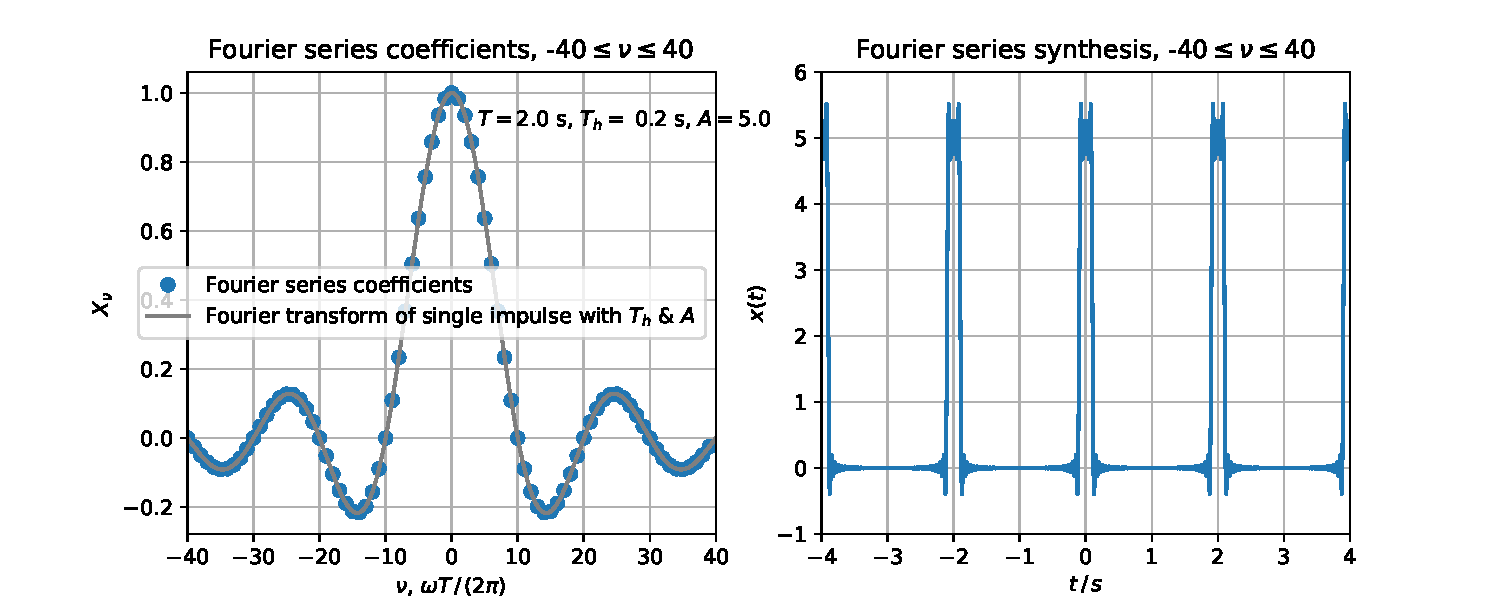
\includegraphics[width=\textwidth]{../fs/D1483A84E2_0.pdf}
\caption{Koeffizienten der komplexen Fourierreihe $c_k$ (links) und Synthese $x(t)$ (rechts) für
$T=1$ s, $T_h=0.1$ s, $A=1/T_h$. \texttt{FourierSeries\_D1483A84E2.ipynb}}
\label{fig:D1483A84E2_0}
\end{figure}

\begin{figure}
\includegraphics[width=\textwidth]{../fs/D1483A84E2_1.pdf}
\caption{Koeffizienten der komplexen Fourierreihe $c_k$ (links) und Synthese $x(t)$ (rechts) für
$T=1$ s, $T_h=0.2$ s, $A=1/T_h$. \texttt{FourierSeries\_D1483A84E2.ipynb}}
\label{fig:D1483A84E2_1}
\end{figure}

\begin{figure}
\includegraphics[width=\textwidth]{../fs/D1483A84E2_2.pdf}
\caption{Koeffizienten der komplexen Fourierreihe $c_k$ (links) und Synthese $x(t)$ (rechts) für
$T=1$ s, $T_h=0.5$ s, $A=1/T_h$. \texttt{FourierSeries\_D1483A84E2.ipynb}}
\label{fig:D1483A84E2_2}
\end{figure}

\begin{figure}
\includegraphics[width=\textwidth]{../fs/D1483A84E2_3.pdf}
\caption{Koeffizienten der komplexen Fourierreihe $c_k$ (links) und Synthese $x(t)$ (rechts) für
$T=1$ s, $T_h=0.8$ s, $A=1/T_h$. \texttt{FourierSeries\_D1483A84E2.ipynb}}
\label{fig:D1483A84E2_3}
\end{figure}

\begin{figure}
\includegraphics[width=\textwidth]{../fs/D1483A84E2_4.pdf}
\caption{Koeffizienten der komplexen Fourierreihe $c_k$ (links) und Synthese $x(t)$ (rechts) für
$T=1$ s, $T_h=1$ s, $A=1/T_h$. \texttt{FourierSeries\_D1483A84E2.ipynb}}
\label{fig:D1483A84E2_4}
\end{figure}




\newpage
\subsection{Fourier-Transformation Beispiel Rechteckfunktion}
\label{sec:8C3958BE4F}
\begin{Ziel}
Wir wollen für die Fouriertransformation die wichtige Dualität zwischen der
Rechteckfunktion und der Spaltfunktion anhand eines fundamentalen Beispiels erfassen.
Zudem enthält auch hier die ausführliche Rechnung Schritte und Umformungen
welche wir wiederkehrend brauchen werden.
\end{Ziel}
\textbf{Aufgabe} {\tiny 8C3958BE4F}: Berechnen Sie die Fourier-Transformation für
\begin{itemize}
\item axialsymmetrische Rechteckfunktion der Breite $T_h$ und Amplitude $A$
\end{itemize}

\begin{figure}[h!]
\centering
\begin{tikzpicture}[domain=0:2]
\draw[->] (-2,0) -- (2,0) node[below right] {$t$};
\draw[->] (0,0) -- (0,1.5) node[above] {$x(t)$};
\draw[-, C0, ultra thick] (-2,0) -- (-0.5,0) node[below] {$\frac{-T_h}{2}$} -- (-0.5,1) node[left] {$A$} -- (0.5,1) -- (0.5,0) node[below] {$\frac{+T_h}{2}$} -- (2,0);
\end{tikzpicture}
\end{figure}

\begin{Werkzeug}
Synthese mit Fouriertransformation
\begin{align}
x(t) = \frac{1}{2\pi} \int\limits_{-\infty}^{+\infty} X(\im\omega) \, \e^{+\im \omega t} \fsd \omega
\end{align}
%
Analyse mit Fouriertransformation
\begin{align}
X(\im \omega) = \int\limits_{-\infty}^{+\infty} x(t) \, \e^{-\im \omega t} \fsd t
\end{align}
\end{Werkzeug}

\begin{Ansatz}
\begin{equation}
X(\im \omega) = \int\limits_{-T_h/2}^{+T_h/2} A \e^{-\im \omega t} \mathrm{d}t
\end{equation}
\end{Ansatz}

\begin{ExCalc}
Integrieren
\begin{equation}
X(\im \omega) = A \frac{\e^{-\im \omega t}}{-\im \omega} \bigg|_{-T_h/2}^{+T_h/2}
\end{equation}
Grenzen einsetzen
\begin{equation}
X(\im \omega) = A \frac{\e^{-\im \omega T_h/2}-\e^{+\im \omega T_h/2}}{-\im \omega}
\end{equation}
Vorzeichen
\begin{equation}
X(\im \omega) = A \frac{\e^{+\im \omega T_h/2}-\e^{-\im \omega T_h/2}}{\im \omega}
\end{equation}
Erweitern mit dem Ziel $\sin(x) = \frac{\e^{+\im x}-\e^{-\im x}}{2\im}$, $\mathrm{sinc}(x):=\frac{\sin(x)}{x}$
\begin{equation}
X(\im \omega) = A \frac{\e^{+\im \omega T_h/2}-\e^{-\im \omega T_h/2}}{\im \omega} \frac{T_h/2}{T_h/2} \cdot \frac{2}{2}
\end{equation}
Umsortieren
\begin{equation}
X(\im \omega) = A \frac{\e^{+\im \omega T_h/2}-\e^{-\im \omega T_h/2}}{2 \im \omega T_h/2} \frac{T_h/2}{1} \cdot \frac{2}{1}
\end{equation}
\end{ExCalc}

\begin{Loesung}
\begin{equation}
\label{eq:8C3958BE4F_Loesung}
X(\im \omega) = A T_h \cdot \mathrm{sinc}(\omega \frac{T_h}{2})
\end{equation}

Wir bekommen wieder eine Spaltfunktion, wie schon bei der Fourierreihe aus Aufgabe
\ref{sec:D1483A84E2}, vgl. \eq{eq:D1483A84E2_Loesung}.
%
Diesmal, weil die Frequenzvariable $\omega$ kontinuierlich ist,
wird die Spaltfunktion 'überall' ausgewertet,
die Fouriertransformation ist also eine kontinuierliche Funktion über $\omega$.
%
Auch hier ist $X(\im\omega)\in\mathbb{R}$ ein Spezialfall.
%
Der Faktor $\frac{T_h}{2}$ im sinc-Argument bestimmt wieder die Breite der
Spaltfunktion.

Merke bzw. besser sieh in den Formeln:

Je \textbf{kleiner} $T_h$, also je \textbf{schmal}er der
\textbf{Rechteck}impuls, desto \textbf{breit}er die \textbf{Spalt}funktion.

Je \textbf{größer} $T_h$, also je \textbf{breit}er der
\textbf{Rechteck}impuls, desto \textbf{schmal}er die \textbf{Spalt}funktion.
%
Dieser Zusammenhang ist fundamental in der Signalverarbeitung und der
Kommunikationstechnik und wurde in \fig{fig:8C3958BE4F} grafisch aufbereitet.

Was erwarten wir für $T_h\to 0$ (idealer Impuls) und was für $T_h\to \infty$
(Gleichspannung)? In beiden Fällen bekommen
wir Probleme beim Integrieren. Aber dies sind in der SigSys überaus wichtige
Grenzfälle, für die auch Fouriertransformierte existieren. Wir werden sie bald
kennenlernen.

Wir werden in der VL und UE sehr oft das Elementarsignal

\begin{equation}
\text{rect}(t) := \begin{cases} 1 & |t| < \frac{1}{2} \\ \frac{1}{2} & |t| = \frac{1}{2} \\ 0 & |t| > \frac{1}{2} \end{cases}\quad,
\end{equation}
also den Rechteckimpuls mit $T_h=1$ und $A=1$, zum Rechnen benutzen.
%
Die Fouriertransformierte von $\text{rect}(t)$ lautet dann abgeleitet aus
\eq{eq:8C3958BE4F_Loesung} einfach
$X(\im \omega) = \mathrm{sinc}(\frac{\omega}{2})$.
%
Eine oft benutzte Schreibweise von Fouriertransformationspaaren (sogenannte
Korrespondenzen, siehe Formelsammlung) benutzt den Operator $\laplace$.
%
Wir schreiben für das soeben gefundene Transformationspaar
\begin{equation}
x(t) = \text{rect}(t) \quad \laplace \quad X(\im \omega) = \mathrm{sinc}(\frac{\omega}{2})
\end{equation}
%
Eine weitere Korrespondenz ist
\begin{equation}
x(t) = \text{sinc}(t) \quad \laplace \quad X(\im \omega) = \pi \, \mathrm{rect}(\frac{\omega}{2}),
\end{equation}
also bis auf den Faktor $\pi$ vertauscht.
%Diese Korrespondenz direkt zu
%beweisen, also die Spaltfunktion fourierzutransformieren ist nicht trivial, aber
%man kann die inverse Fourier Transformation berechnen. Das ist wieder nur der
%Rechteckimpuls unter dem Integralkern.
%
Die Dualität, also \textbf{Spaltfunktion transformiert ergibt Rechteckfunktion und umgekehrt},
dürfen wir die ganze Zeit nicht aus den Augen verlieren. Das ist so ein bisschen
wie der Satz des Pythagoras bei rechtwinkligen Dreiecken, ohne den wird's auch eher
dünne Rechnerei mit wenig Vertändnis.

Schauen wir noch kurz zurück in die \fig{fig:D1483A84E2_0} bis \fig{fig:D1483A84E2_4}.
Dort wurde in grau immer der Verlauf der hier diskutierten Fouriertransformierten
hinterlegt. Man sieht, dass die Werte der Fourierkoeffizienten $T \cdot c_k$
\eq{eq:D1483A84E2_Loesung} aus Aufgabe \ref{sec:D1483A84E2}
mit den Werten von $X(\im\omega)$ \eq{eq:8C3958BE4F_Loesung} übereinstimmen bei
$\omega_0 k = \omega$. Dies ist kein Zufall. Das werden wir später als Abtastung
kennenlernen.



\end{Loesung}

\begin{figure*}[h!]
\centering
\begin{subfigure}{1\textwidth}
\centering
\includegraphics[width=\textwidth]{../ft/8C3958BE4F_1.pdf}
\caption{Rechteckimpulse für verschiedene $T_h$ und gewähltem $A=1/T_h$.
Achtung: Um die resultierenden Amplitudenunterschiede sinnvoll darstellen zu können,
ist $\log_{10}x(t)$ über $t$ aufgetragen. Da $\log_{10}(0)=-\infty$
ist nur der Signalteil mit (positiver) Amplitude $A=1/T_h$ sichtbar.}
\label{fig:8C3958BE4F_1}
\end{subfigure}
\\
\begin{subfigure}{1\textwidth}
\centering
\includegraphics[width=\textwidth]{../ft/8C3958BE4F_0.pdf}
\caption{Fouriertransformation der Rechteck-Impulse aus
\fig{fig:8C3958BE4F_1}. Durch die Wahl $A=1/T_h$ haben alle Rechteckimpulse Fläche
1 und alle Fouriertransformierten
das gleiche globale Maximum (bei $\omega=0$ rad/s) mit Wert 1.}
\label{fig:8C3958BE4F_0}
\end{subfigure}
%
\caption{Rechteckimpulse (oben) und Fouriertransformierte (unten).
Liniendickenvariation zu besseren Unterscheidbarkeit bei Graustufenanzeige.
\texttt{FourierTransformation\_8C3958BE4F.ipynb}}
\label{fig:8C3958BE4F}
\end{figure*}


\begin{figure}[h!]
\includegraphics[width=\textwidth]{../ft/8C3958BE4F_SingleCase_MagPhase.pdf}
  \caption{Betrag (oben) und Phase (unten) der rellwertigen
  Fouriertransformierten \eq{eq:8C3958BE4F_Loesung}. Für eine Variable
  $a\in\mathbb{R}$ gilt $a = -a \e^{\pm\im\pi}$, daher
  die Phasensprünge um $\pm\pi$ zum punktsymmetrisches Spektrum
  bei negativer Amplitude der Spaltfunktion.
\texttt{FourierTransformation\_8C3958BE4F.ipynb}}
  \label{fig:8C3958BE4F_SingleCase_MagPhase}
\end{figure}




\clearpage
\subsection{Fourier-Transformation Signal-Verschiebung}
\label{sec:A8A2DEE53A}
\begin{Ziel}
Wir wollen uns erarbeiten, wie sich eine Zeitverschiebung des Signals auf die
Fouriertransformierte auswirkt und damit das sogenannte Verschiebungsgesetz
kennenlernen und/oder wiederholen.
Merke bzw. besser sieh in den Formeln:
Zeitverschiebung bedeutet immer Phasenänderung in der Fouriertransformierten.
\end{Ziel}
\textbf{Aufgabe} {\tiny A8A2DEE53A}: Berechnen Sie die Fourier-Transformation für
\begin{itemize}
\item dargestellte Rechteckfunktion der Breite $T_h$ und Amplitude $A$
\end{itemize}
%
\begin{figure}[h!]
\centering
\begin{tikzpicture}[domain=0:2]
\draw[->] (-2,0) -- (2,0) node[below right] {$t$};
\draw[->] (0,0) -- (0,1.5) node[above] {$x(t)$};
\draw[-, C0, ultra thick] (-2,0) -- (-0.0,0) node[below] {$0$} -- (-0,1) node[left] {$A$} -- (1,1) -- (1,0) node[below] {$T_h$} -- (2,0);
\end{tikzpicture}
\end{figure}
%
Wir erkennen die in Aufgabe \ref{sec:8C3958BE4F} hier um $T_h/2$, also nach rechts,
verschobene Rechteckfunktion.


\begin{Werkzeug}
nothing new here...wir machen
Analyse mit Fouriertransformation
\begin{align}
X(\im \omega) = \int\limits_{-\infty}^{+\infty} x(t) \, \e^{-\im \omega t} \fsd t
\end{align}
\end{Werkzeug}
\begin{Ansatz}
\begin{equation}
X(\im \omega) = \int\limits_{0}^{T_h} A \e^{-\im \omega t} \mathrm{d}t
\end{equation}
\end{Ansatz}


\begin{ExCalc}
Integrieren
\begin{equation}
X(\im \omega) = A \frac{\e^{-\im \omega t}}{-\im \omega} \bigg|_{0}^{T_h}
\end{equation}
Grenzen einsetzen
\begin{equation}
X(\im \omega) = A \frac{\e^{-\im \omega T_h}-1}{-\im \omega}
\end{equation}
Vorzeichen
\begin{equation}
X(\im \omega) = A \frac{1 - \e^{-\im \omega T_h}}{\im \omega}
\end{equation}
Erweitern mit dem Ziel $\sin(x) = \frac{\e^{+\im x}-\e^{-\im x}}{2\im}$, $\mathrm{sinc}(x):=\frac{\sin(x)}{x}$
\begin{equation}
X(\im \omega) = A \frac{1 - \e^{-\im \omega T_h}}{\im \omega} \underbrace{\e^{+\im\omega\frac{T_h}{2}} \e^{-\im\omega\frac{T_h}{2}}}_{=1}=
A \frac{\e^{+\im\omega\frac{T_h}{2}} - \e^{-\im\omega\frac{T_h}{2}}}{\im\omega} \e^{-\im\omega\frac{T_h}{2}}
\end{equation}
\begin{equation}
X(\im \omega) = A \frac{\e^{+\im\omega\frac{T_h}{2}} - \e^{-\im\omega\frac{T_h}{2}}}{\im\omega} \e^{-\im\omega\frac{T_h}{2}}
\cdot \frac{T_h/2}{T_h/2} \cdot \frac{2}{2}
\end{equation}
Umsortieren
\begin{equation}
X(\im \omega) = A T_h \frac{\e^{+\im\omega\frac{T_h}{2}} - \e^{-\im\omega\frac{T_h}{2}}}{2 \im \cdot \omega T_h/2} \e^{-\im\omega\frac{T_h}{2}} =
A T_h \frac{\sin(\omega\frac{T_h}{2})}{\omega\frac{T_h}{2}} \e^{-\im\omega\frac{T_h}{2}}
\end{equation}
\end{ExCalc}


\begin{Loesung}
\begin{equation}
\label{eq:A8A2DEE53A_Loesung}
X(\im \omega) = A T_h \cdot \mathrm{sinc}(\omega\frac{T_h}{2}) \cdot  \e^{-\im\omega\frac{T_h}{2}}
\end{equation}
%
Wir erkennen, dass \eq{eq:8C3958BE4F_Loesung} um den komplexen Dreher / Zeiger $\e^{-\im\omega\frac{T_h}{2}}$
erweitert wird und nun $X(\im \omega)\in\mathbb{C}$.
%
Wir müssen bei grafischen Darstellungen daher eigentlich streng immer mindest
zwei Diagramme anfertigen:
\begin{itemize}
  \item Realteil + Imaginärteil und/oder
  \item Betrag + Phase
\end{itemize}
%
Eine Darstellung in Betrag und Phase ist üblich, weil dies bei praktischen
Problemen, schnell hilfreiche Informationen offenbart. Das haben wir auch schon
bei der komplexen Wechselstromrechnung benutzt.


Im Gegensatz zum vorherigen Beispiel und \fig{fig:8C3958BE4F_SingleCase_MagPhase},
wo $X(\im \omega)\in\mathbb{R}<0$ Phasensprünge um $\pi$ verursacht haben, müssen
wir hier eine stückweise stetige, linear Phasenfunktion $\phi(\omega)$ berücksichtigen.
Schauen wir schonmal auf \fig{fig:A8A2DEE53A} unten, um uns ein Bild zu machen.
%
Der Anstieg der Geradenteile lässt sich direkt aus dem komplexen Dreher rauslesen
zu $-\frac{T_h}{2}$.
%
Für die Fouriertransformierte in Betrag und Phase dargestellt, gilt mit $k\in\mathbb{Z}$
\begin{equation}
X(\im \omega) = \bigg|A T_h \cdot \mathrm{sinc}(\omega\frac{T_h}{2})\bigg|
\cdot  \e^{-\im\omega\frac{T_h}{2}}\cdot
\begin{cases}
\e^{\im (0+2\pi k)}\quad \text{für}\quad \mathrm{sinc}(\omega\frac{T_h}{2})\geq0\\
\e^{\im (\pi + 2\pi k)}\quad \text{für}\quad\mathrm{sinc}(\omega\frac{T_h}{2})<0.
\end{cases}
\end{equation}
Überall da wo die Spaltfunktion einen Polaritärswechsel macht, entsteht
eine Phasen-Unstetigkeitstelle, weil die Phase springt um $\pi$ bzw. wegen der
$2\pi$-Vieldeutigkeit um $\pi + 2\pi k$.
%
Die Phasenfunktion ist daher
\begin{equation}
\phi(\omega) = -\omega\frac{T_h}{2} +
\begin{cases}
2\pi k\quad \text{für}\quad \mathrm{sinc}(\omega\frac{T_h}{2})\geq0\\
\pi + 2\pi k\quad \text{für}\quad\mathrm{sinc}(\omega\frac{T_h}{2})<0,
\end{cases}
\end{equation}
Die numpy-Funktion \verb|angle()| wertet die Phase zwischen $-\pi$ und $+\pi$ aus,
deswegen bekommen wir den in \fig{fig:A8A2DEE53A} dargestellten Verlauf der Phase.

Daher nochmal: Jenseits der Phasensprünge, ist zu realisieren, dass
eine zeitliche Verschiebung um $\frac{T_h}{2}$ in der Fouriertransformierten
zu einer Phasenänderung mit Anstieg $-\frac{T_h}{2}$ (negativ, fallend)
führt und der Betrag erhalten bleibt.
%
In \fig{fig:A8A2DEE53A} ist daher das Verhalten von \eq{eq:A8A2DEE53A_Loesung} als
Betrag und Phase über $\omega$ dargestellt.

Der Betrag der Spaltfunktion ist einfach zu erhalten: wir klappen einfach alle
negativen Funktionswerte in Richtung positiver Ordinate.
%
Die Phase ist die stückweise stetig Gerade über $\omega$ durch den Ursprung
mit Anstieg $-T_h/2$, also fallend.
%
Diese \textbf{Phase}nfunktion ist bzgl. des Ursprungs \textbf{punktsymmetrisch}.
Dies gilt immer für die Fouriertransformierten $X(\im\omega)$ von \textbf{reellwertigen}
Signalen $x(t)$.
%
Größere Zeitverschiebung $T_h/2$ bedeutet größere Phasenverschiebung, also steilere
fallende Geradenstücke.

Das was wir anhand eines speziellen (wichtigen) Beispiels gezeigt haben, gilt auch
allgemein. Die Korrespondenz zur \textbf{Zeitverschiebung} um $\tau\in\mathbb{R}$
---bekannt als \textbf{Verschiebungssatz}---lautet
\begin{align}
x(t) & \quad \laplace \quad X(\im\omega)\\
x(t - \tau) & \quad \laplace \quad X(\im\omega) \cdot \e^{-\im\omega \tau}.
\end{align}
%
Man kann natürlich auch eine Fouriertransformierte um die Kreisfrequenz
$\omega_0\in\mathbb{R}$ verschieben, vgl. Aufgabe \ref{sec:9D652BE72B}.
%
Die Korrespondenz zur \textbf{Frequenzverschiebung}
---bekannt als \textbf{Modulationssatz}---lautet
\begin{align}
x(t) & \quad \laplace \quad X(\im\omega)\\
\label{eq:A8A2DEE53A_ModTheoremTime}
x(t) \cdot \e^{+\im\omega_0 t} & \quad \laplace \quad X(\im[\omega-\omega_0]).
\end{align}
%
Bemerkenswert ist der gekreuzte Zusammenhang Zeit-/ Frequenzverschiebung
vs.
Frequenz-/ Zeitmodulation,
jedoch mit anderem Vorzeichen
in im komplexen Dreher.
\end{Loesung}

\begin{figure}[h!]
\centering
\includegraphics[width=0.9\textwidth]{../ft/A8A2DEE53A.pdf}
  \caption{Betrag (oben) und Phase (unten) der Fouriertransformierten \eq{eq:A8A2DEE53A_Loesung}.
\textbf{Vorsicht:} Die Grafik suggeriert, dass eine zeitliche Rechts-Verschiebung
sowohl Phase als auch Betrag ändert. Dies passiert aber hier speziell, weil wir in der
Aufgabe nach einer Verschiebung um $T_h/2$ gefragt haben, und $T_h$
im Argument der Spaltfunktion die Breite dieser bestimmt.
\texttt{FourierTransformation\_A8A2DEE53A.ipynb}}
  \label{fig:A8A2DEE53A}
\end{figure}


\clearpage
\subsection{Fourier-Transformation Signal-Zeitumkehr}
\label{sec:1CFE5FE3A1}
\begin{Ziel}
Wir wollen uns erarbeiten, wie sich eine Zeitumkehr in der Fouriertransformierten
auswirkt und dabei eine wichtige Symmetrie der Korrespondenzen kennenlernen.

Merke bzw. besser sieh in den Formeln: Zeitumkehr ist Phasenumkehr in der Fouriertransformierten.
\end{Ziel}

\textbf{Aufgabe} {\tiny 1CFE5FE3A1}: Berechnen Sie die Fourier-Transformation für
\begin{itemize}
\item dargestellte Rechteckfunktion der Breite $T_h$ und Amplitude $A$
\end{itemize}
%
\begin{figure}[h!]
\centering
\begin{tikzpicture}[domain=0:2]
\draw[->] (-2,0) -- (2,0) node[below right] {$t$};
\draw[->] (0,0) -- (0,1.5) node[above] {$x(t)$};
\draw[-, C0, ultra thick] (-2,0) -- (-1,0) node[below] {$-T_h$} -- (-1,1) node[left] {$A$} -- (0,1) -- (0,0) -- (2,0);
\end{tikzpicture}
\end{figure}
%
Wir erkennen
\begin{itemize}
\item die in Aufgabe \ref{sec:8C3958BE4F} hier um $-T_h/2$, also nach links,
verschobene Rechteckfunktion
\item die in Aufgabe \ref{sec:A8A2DEE53A} hier zeitgedrehte Rechteckfunktion
\end{itemize}

\begin{Werkzeug}
Korrespondenz Zeitverschiebung um $\tau\in\mathbb{R}$:
\begin{align}
x(t) & \quad \laplace \quad X(\im\omega)\\
x(t - \tau) & \quad \laplace \quad X(\im\omega) \cdot \e^{-\im\omega \tau}.
\end{align}
Analyse mit Fouriertransformation:
\begin{align}
X(\im \omega) = \int\limits_{-\infty}^{+\infty} x(t) \, \e^{-\im \omega t} \fsd t
\end{align}
\end{Werkzeug}

\begin{Ansatz}
Mit Kenntnis der Fouriertransformierten aus Aufgabe \ref{sec:8C3958BE4F}, d.h. der
unverschobenen Zeitfunktion, können wir den Zeitverschiebungssatz anwenden:

\begin{equation}
x(t - (-T_h/2)) \quad \laplace \quad X(\im\omega) \cdot \e^{-\im\omega (-T_h/2)}
\end{equation}
Das Endergebnis für die hier gestellte Aufgabe lautet daher
\begin{equation}
X(\im \omega) = A T_h \cdot \mathrm{sinc}(\omega\frac{T_h}{2}) \cdot  \e^{+\im\omega\frac{T_h}{2}}.
\end{equation}
Wir können aber auch wieder zu Fuß das Integral der Fourier Transformation
\begin{equation}
X(\im \omega) = \int\limits_{-T_h}^{0} A \e^{-\im \omega t} \mathrm{d}t
\end{equation}
mit ähnlichem Vorgehen wie Aufgabe \ref{sec:A8A2DEE53A} lösen und müssen das
gleiche Endergebnis bekommen, wie die folgende ausführliche Rechnung zeigt.
\end{Ansatz}
\begin{ExCalc}
%Integrieren
\begin{equation}
X(\im \omega) = A \frac{\e^{-\im \omega t}}{-\im \omega} \bigg|_{-T_h}^{0}
\end{equation}
%Grenzen einsetzen
\begin{equation}
X(\im \omega) = A \frac{1 - \e^{+\im \omega T_h}}{-\im \omega}
\end{equation}
%Vorzeichen
\begin{equation}
X(\im \omega) = A \frac{\e^{+\im \omega T_h}-1}{\im \omega}
\end{equation}
%Erweitern mit dem Ziel $\sin(x) = \frac{\e^{+\im x}-\e^{-\im x}}{2\im}$, $\mathrm{sinc}(x):=\frac{\sin(x)}{x}$
\begin{equation}
X(\im \omega) = A \frac{\e^{+\im \omega T_h}-1}{\im \omega} \underbrace{\e^{-\im\omega\frac{T_h}{2}} \e^{+\im\omega\frac{T_h}{2}}}_{=1}=
A \frac{\e^{+\im\omega\frac{T_h}{2}} - \e^{-\im\omega\frac{T_h}{2}}}{\im\omega} \e^{+\im\omega\frac{T_h}{2}}
\end{equation}
\begin{equation}
X(\im \omega) = A \frac{\e^{+\im\omega\frac{T_h}{2}} - \e^{-\im\omega\frac{T_h}{2}}}{\im\omega} \e^{+\im\omega\frac{T_h}{2}}
\cdot \frac{T_h/2}{T_h/2} \cdot \frac{2}{2}
\end{equation}
%Umsortieren
\begin{equation}
X(\im \omega) = A T_h \frac{\e^{+\im\omega\frac{T_h}{2}} - \e^{-\im\omega\frac{T_h}{2}}}{2 \im \cdot \omega T_h/2} \e^{+\im\omega\frac{T_h}{2}} =
A T_h \frac{\sin(\omega\frac{T_h}{2})}{\omega\frac{T_h}{2}} \e^{+\im\omega\frac{T_h}{2}}
\end{equation}
\end{ExCalc}
\begin{Loesung}
Das Ergebnis
\begin{equation}
\label{eq:1CFE5FE3A1_Loesung}
X(\im \omega) = A T_h \cdot \mathrm{sinc}(\omega\frac{T_h}{2}) \cdot  \e^{+\im\omega\frac{T_h}{2}}.
\end{equation}
ist in \fig{fig:1CFE5FE3A1} dargestellt. Der Betrag
$\bigg|A T_h \cdot \mathrm{sinc}(\omega\frac{T_h}{2})\bigg|$
ist gleich wie in Aufgabe \ref{sec:A8A2DEE53A}, weil wir gelernt haben, dass
eine Zeitverschiebung nur die Phase in der Fouriertransformierten ändert.
%

Der wichtige neue Punkt ist, dass bei zeitlicher Linksverschiebung (Voreilen)
die \textbf{unstetige Phasenfunktion} $\phi(\omega)$
\textbf{diesmal ansteigend} ist,  da
\begin{equation}
X(\im \omega) = \bigg|A T_h \cdot \mathrm{sinc}(\omega\frac{T_h}{2})\bigg|
\cdot  \e^{+\im\omega\frac{T_h}{2}}\cdot
\begin{cases}
\e^{\im (0+2\pi k)}\quad \text{für}\quad \mathrm{sinc}(\omega\frac{T_h}{2})\geq0\\
\e^{\im (\pi + 2\pi k)}\quad \text{für}\quad\mathrm{sinc}(\omega\frac{T_h}{2})<0.
\end{cases}
\end{equation}

\begin{equation}
\phi(\omega) = +\omega\frac{T_h}{2} +
\begin{cases}
2\pi k\quad \text{für}\quad \mathrm{sinc}(\omega\frac{T_h}{2})\geq0\\
\pi + 2\pi k\quad \text{für}\quad\mathrm{sinc}(\omega\frac{T_h}{2})<0,
\end{cases}
\end{equation}
Die Phase ist eine stückweise stetige Geradengleichung über $\omega$ durch den
Ursprung und mit Anstieg $+T_h/2$, also diesmal steigend!
%
Die \textbf{Zeitumkehr} erzeugt also eine \textbf{Phasenumkehr}, vgl.
Aufgabe \ref{sec:A8A2DEE53A} fallende Phase, Aufgabe \ref{sec:1CFE5FE3A1} hier steigende Phase.
%
Dies gilt auch wieder verallgemeinert und ist eine wichtige \textbf{Symmetrie}eigenschaft
der Fourier Transformation
%
\begin{align}
x(+t) \quad \laplace \quad X(+\im\omega) =& |X(\im\omega)| \, \e^{+\im\angle X(\im\omega)}\\
x(-t) \quad \laplace \quad X(-\im\omega) =& |X(\im\omega)| \, \e^{-\im\angle X(\im\omega)}
\end{align}
%
Zufällig (naja, die Aufgabe war so gewählt)
in unserem Beispiel konnten wir das Problem auch über Zeitverschiebung
lösen, weil wir die unverschobene Rechteckfunktion bereits gut kennen.
\end{Loesung}
%
\begin{figure}[h!]
\includegraphics[width=\textwidth]{../ft/1CFE5FE3A1.pdf}
  \caption{Betrag (oben) und Phase (unten) der Fouriertransformierten \eq{eq:1CFE5FE3A1_Loesung}.
\textbf{Erneut Vorsicht:} Die Grafik suggeriert, dass eine zeitliche Links-Verschiebung
sowohl Phase als auch Betrag ändert. Dies passiert aber hier speziell, weil wir in der
Aufgabe nach einer Verschiebung um $-T_h/2$ gefragt haben, und $T_h$
im Argument der Spaltfunktion die Breite dieser bestimmt.
\texttt{FourierTransformation\_1CFE5FE3A1.ipynb}}
  \label{fig:1CFE5FE3A1}
\end{figure}





\clearpage
\subsection{Fourier-Transformation Signal-Modulation}
\label{sec:9D652BE72B}
\begin{Ziel}
Anhand eines speziellen Beispiels erfassen wir das Wesen des Modulationstheorems.
\end{Ziel}
\textbf{Aufgabe} {\tiny 9D652BE72B}: Berechnen Sie die Fouriertransformation für
\begin{itemize}
\item axialsymmetrische Rechteckfunktion der Breite $T_h$ und Amplitude $A$
\item die mit der komplexen Schwingung $\e^{+\im \omega_0 t}$ mit Kreisfrequenz $\omega_0>0$
multipliziert wird
\end{itemize}
Wir wollen die Fouriertransformation Korrespondenz \eq{eq:A8A2DEE53A_ModTheoremTime}
\begin{align}
x(t) \cdot \e^{+\im\omega_0 t} & \quad \laplace \quad X(\im[\omega-\omega_0])
\end{align}
nochmal am Beispiel sehen.

\begin{figure}[h!]
\centering
\begin{tikzpicture}[domain=0:2]
\draw[->] (-2,0) -- (2,0) node[below right] {$t$};
\draw[->] (0,0) -- (0,1.5) node[above] {$x(t)$};
\draw[-, C0, ultra thick] (-2,0) -- (-0.5,0) node[below] {$\frac{-T_h}{2}$} -- (-0.5,1) node[left] {$A$} -- (0.5,1) -- (0.5,0) node[below] {$\frac{+T_h}{2}$} -- (2,0);
\end{tikzpicture}
\end{figure}

\begin{Werkzeug}
Analyse mit Fouriertransformation
\begin{align}
X(\im \omega) = \int\limits_{-\infty}^{+\infty} x(t) \, \e^{-\im \omega t} \fsd t
\end{align}
\end{Werkzeug}
\begin{Ansatz}
\begin{align}
X_m(\im \omega) = \int\limits_{-T_h/2}^{+T_h/2} \e^{+\im \omega_0 t} \cdot A \, \e^{-\im \omega t} \mathrm{d}t
\end{align}
\end{Ansatz}
\begin{ExCalc}
\begin{align}
X_m(\im \omega) = A \int\limits_{-T_h/2}^{+T_h/2} \e^{-\im (\omega-\omega_0) t} \mathrm{d}t =
A \frac{\e^{-\im (\omega-\omega_0) t}}{-\im (\omega-\omega_0)}\bigg|_{-T_h/2}^{+T_h/2} =
A \frac{\e^{-\im (\omega-\omega_0) T_h/2} - \e^{+\im (\omega-\omega_0) T_h/2}}{-\im (\omega-\omega_0)}
\end{align}
Vorzeichen drehen, erweitern, $\sin(x) = \frac{\e^{+\im x}-\e^{-\im x}}{2\im}$, $\mathrm{sinc}(x):=\frac{\sin (x)}{x}$
\begin{align}
X_m(\im \omega) = A \frac{\e^{+\im (\omega-\omega_0) T_h/2} - \e^{-\im (\omega-\omega_0) T_h/2}}{\im (\omega-\omega_0)} \cdot \frac{T_h/2}{T_h/2} \cdot \frac{2}{2}
\end{align}
\end{ExCalc}
\begin{Loesung}
\begin{align}
X_m(\im \omega) = A T_h \cdot \mathrm{sinc}\left((\omega-\omega_0) \frac{T_h}{2}\right)
\end{align}
Wir können mit Vergleich dieser und  Aufgabe \ref{sec:8C3958BE4F} beobachten, dass
die Korrespondenz
\begin{align}
\e^{+\im \omega_0 t} \cdot x(t) \quad\laplace\quad X\left(\im [\omega-\omega_0]\right)
\end{align}
gilt.
%
Dieser Zusammenhang gilt generell und ist als Modulationstheorem der
Fourier Transformation bekannt.
%
Das Spektrum (die Fouriertransformierte) $X(\im \omega)$ wird im Frequenzbereich
um $\omega_0$ verschoben, wenn $x(t)$ mit der komplexen Trägerschwingung
$\e^{+\im \omega_0 t}$ multipliziert wird. In der Nachrichtentechnik bezeichnet man
diesen Vorgang als Modulation von $x(t)$ auf den Träger $\e^{+\im \omega_0 t}$.
Dies benutzt man um Spektren in einen anderen (freien) Frequenzbereich zu
verschieben. Das werden wir bald im Detail besser verstehen.
\end{Loesung}


\begin{mdframed}
\textit{Ausblick:}
%
\\\noindent Wir könnten an dieser Stelle durchaus schon in der Lage sein, uns die
Fouriertransformierten von $x(t) = \cos(\omega_0 t)$ und $x(t) = \sin(\omega_0 t)$
abzuleiten und in Betrag und Phase zu skizzieren.
%
Dazu ist es nicht ratsam, dass Transformationsintegral lösen zu wollen,
es konvergiert nicht, sondern die bisher bekannten Korrespondenzen zusammen
mit den Euler Identitäten
\begin{align}
\cos(\omega_0 t) = \frac{\e^{+\im\omega_0 t}+\e^{-\im\omega_0 t}}{2}\qquad
\sin(\omega_0 t) = \frac{\e^{+\im\omega_0 t}-\e^{-\im\omega_0 t}}{2\im}
\end{align}
zu benutzen.
%
Diese Idee durchzieht die SigSys: `Suchen nach` und `Arbeiten mit` passenden
Korrespondenzen. Wir werden als Ingenieur*innen sehr wahrscheinlich keine unbekannte
Fouriertransformierte neu finden! Überlassen wir dieses Feld hier zunächst
den Integralnerds (vgl. \cite{Abramowitz1972}, \cite{Gradshteyn2007}) und lernen
stattdessen was wir mit den Tools anstellen können und was sie uns im Wesen sagen.
\end{mdframed}

%
In den bisherigen Aufgaben haben wir uns mit einfachen Signalen und der
Fouriertransformierten beschäftigt, sprich wir haben geschaut, welche Frequenzen
stecken mit welcher Amplitude in den untersuchten Signalen.
%
Als Spezialfall bekamen wir für periodische Signale Fourierkoeffizienten.
%
Das ist der \textbf{SigSys-Teil: Signalanalyse und -synthese}. Wir werden insgesamt
\textbf{vier Fouriertransformationen} kennenlernen, alle spezialisiert auf bestimmte
Signaltypen, zwei kennen wir nun schon ein wenig besser: Fourierreihe und
Fouriertransformation.
Die anderen beiden sind

\url{https://de.wikipedia.org/wiki/Diskrete_Fourier-Transformation}

\url{https://de.wikipedia.org/wiki/Fouriertransformation_für_zeitdiskrete_Signale}

Die Idee mit Korrespondenzen zu arbeiten, bleibt für alle Transformationen
erhalten. Auch werden wir die Sinc/Rect-Dualitäten immer wieder finden,
genauso wie Zeit-/Frequenzverschiebung.




\begin{comment}
\newpage
\subsection{Fourier-Transformation Cosinus-Schwingung}
\label{sec:610482EF57}
\begin{Ziel}
Mit dem (eigentlich noch recht bescheidenen) Wissen zur Fourier-Transformation
können wir trotzdem schon eine ganze Menge fundamental wichtiger Aspekte ableiten,
diese sind in Büchern bereits bestens abgedeckt.
Es kann jedoch nicht schaden, hin und wieder Sachen neu zu erfinden.
Wir werden die Qualität je schmaler/breiter Rechteckfunktion desto breiter/schmaler
Spaltfunktion erfassen und uns das zunutze machen, um die auf direktem Wege
für uns noch nicht lösbare Aufgabenstellung trotzdem zu lösen.
\end{Ziel}
\textbf{Aufgabe} {\tiny 610482EF57}: Berechnen Sie die Fouriertransformation für
\begin{itemize}
\item Cosinus-Schwingung $\cos(\omega_1 t)$ mit Kreisfrequenz $\omega_1>0$
\end{itemize}
\begin{Werkzeug}
Analyse mit Fouriertransformation
\begin{align}
X(\im \omega) = \int\limits_{-\infty}^{+\infty} x(t) \, \e^{-\im \omega t} \fsd t
\end{align}
\end{Werkzeug}
\begin{Ansatz}
\begin{align}
X(\im \omega) = \int\limits_{-\infty}^{+\infty} \cos(\omega_1 t) \, \e^{-\im \omega t} \fsd t
\end{align}
Dieses Integral konvergiert nicht und suggeriert, dass es keine Lösung gibt, was
natürlich nicht stimmt, sonst gäbe es die Aufgabenstellung nicht. Wir müssen
anders herangehen.
%
Wir könnten $x(t) = \cos(\omega_1 t)$ definieren und das Modulationstheorem
aus vorheriger Aufgabe mit $\omega_0=0$ zu Hilfe nehmen. Das bringt uns nur keinen
Schritt weiter.
%
Wir könnten $x(t) = 1$ definieren und das Modulationstheorem
aus vorheriger Aufgabe mit $\omega_0=\omega_1$ zu Hilfe nehmen. Dann haben wir
zwei Probleme mehr: a) wir kennen die Transformationsregel für die Modulation
mit dem reellen Cosinussignal noch nicht und b) wir kennen die Lösung der
Fourier Transformation des unmodulierten Signals $x(t)=1$, also
\begin{align}
X(\im \omega) = \int\limits_{-\infty}^{+\infty} 1 \e^{-\im \omega t} \fsd t = ?
\end{align}
noch nicht. Es stresst hier wieder, dass das Integral nicht konvergiert. Mit
unendlichen Grenzen können wir hier noch nicht gut umgehen.
%
Benutzen wir also unser Handwerkszeug aus den vorigen Übungen und legen zunächst
eine endliche Integrationsgrenze fest, nämlich mit Hilfe der
axialsymmetrischen Rechteckfunktion der Breite $T$ und Amplitude $A$. Diesen
Rechteckverlauf lassen wir dann immer breiter werden, bis er sich im Grenzfall
von $-\infty$ bis
$+\infty$ erstreckt.
%
Unser Ansatz lautet also
\begin{align}
X(\im \omega) = \int\limits_{-T_h/2}^{+T_h/2} A \cos(\omega_1 t) \, \e^{-\im \omega t} \fsd t
\end{align}
Wir erkennen, dass der Reckteckimpuls auf den Cosinus-Träger moduliert wird, aber
wir kennen das Modulationsgesetz diesbezüglich noch nicht.
Daher lösen wir das Integral zu Fuß.
\end{Ansatz}
\begin{ExCalc}
Wir benutzen $\cos(x) = \frac{1}{2}(\e^{\im x} + \e^{-\im x})$ um
\begin{align}
X(\im \omega) = \int\limits_{-T_h/2}^{+T_h/2} A \frac{1}{2}(\e^{\im \omega_1} + \e^{-\im \omega_1}) \, \e^{-\im \omega t} \fsd t =
\frac{A}{2} \int\limits_{-T_h/2}^{+T_h/2} (\e^{\im \omega_1} + \e^{-\im \omega_1}) \, \e^{-\im \omega t} \fsd t
\end{align}
%
\begin{align}
X(\im \omega) = \int\limits_{-T_h/2}^{+T_h/2} \left(\e^{-\im (\omega-\omega_1) t} + \e^{-\im (\omega+\omega_1) t} \right) \fsd t
\end{align}
%
\begin{align}
X(\im \omega) =
\frac{A}{2} \frac{\e^{-\im (\omega-\omega_1) t}}{-\im (\omega-\omega_1)}\bigg|_{-T_h/2}^{+T_h/2}
+\frac{A}{2} \frac{\e^{-\im (\omega+\omega_1) t}}{-\im (\omega+\omega_1)}\bigg|_{-T_h/2}^{+T_h/2}
\end{align}
%
\begin{align}
X(\im \omega) =
\frac{A}{2} \frac{\e^{-\im (\omega-\omega_1) T_h/2} - \e^{+\im (\omega-\omega_1) T_h/2}}{-\im (\omega-\omega_1)}
+\frac{A}{2} \frac{\e^{-\im (\omega+\omega_1) T_h/2} - \e^{+\im (\omega+\omega_1) T_h/2}}{-\im (\omega+\omega_1)}
\end{align}
%
Vorzeichen, Erweitern
%
\begin{align}
X(\im \omega) =
\frac{A}{2} \frac{\e^{+\im (\omega-\omega_1) T_h/2} - \e^{-\im (\omega-\omega_1) T_h/2}}{\im (\omega-\omega_1)} \cdot \frac{T_h/2}{T_h/2}
+\frac{A}{2} \frac{\e^{+\im (\omega+\omega_1) T_h/2} - \e^{-\im (\omega+\omega_1) T_h/2}}{\im (\omega+\omega_1)} \cdot \frac{T_h/2}{T_h/2}
\end{align}
%
Mit $\sin(x) = \frac{\e^{+\im x}-\e^{-\im x}}{2\im}$, $\mathrm{sinc}(x):=\frac{\sin (x)}{x}$
\begin{align}
X(\im \omega) =
A \frac{T_h}{2} \mathrm{sinc}\left((\omega-\omega_1) \frac{T_h}{2}\right) +
A \frac{T_h}{2} \mathrm{sinc}\left((\omega+\omega_1) \frac{T_h}{2}\right)
\end{align}
Zur Kontrolle: für $\omega_1 = 0$ bekommen wir das Ergebnis aus Aufgabe
\ref{sec:8C3958BE4F}, ein Indiz, dass wir uns nicht verrechnet haben.
\end{ExCalc}
%
\begin{Loesung}
Wir bekommen zwei mit $A \frac{T_h}{2}$ gewichtete Spaltfunktionen,
verschoben um $\pm \omega_1$ auf der Frequenzachse. Das Maximum der ersten Spaltfunktion
liegt bei $+\omega_1$ (positive Frequenz), das Maximum der zweiten Spaltfunktion
liegt bei $-\omega_1$ (negative Frequenz).



Was ist nun mit der ursprünglichen Aufgabe die Fourier Transformierte des Cosinus
zu finden?
%
Wir können sie ehrlicherweise nur mit einem Vorgriff auf kommenden Stoff erarbeiten, das
ist aber so fundamental, dass es sich lohnt, das hier schonmal anzudeuten.
%
Die Grundidee ist bekanntes mathematisches Handwerkszeug: wir lassen
$T_h\to \infty$ gehen. Dann wird sich für beide gewichtete Spaltfunktionen ein
geschlossener Ausdruck finden lassen.

\end{Loesung}

\begin{mdframed}
\textit{Vorgriff}
%
Zunächst nehmen wir unser vorläufiges Endergebnis und schreiben die Spaltfunction
aus
\begin{align}
X(\im \omega) =
A \frac{T_h}{2} \frac{\sin\left((\omega-\omega_1) \frac{T_h}{2}\right)}{(\omega-\omega_1) \frac{T_h}{2}} +
A \frac{T_h}{2} \frac{\sin\left((\omega+\omega_1) \frac{T_h}{2}\right)}{(\omega+\omega_1) \frac{T_h}{2}}
\end{align}
kürzen ein wenig und erweitern mit $\pi$
\begin{align}
X(\im \omega) =
A \pi \frac{\sin\left((\omega-\omega_1) \frac{T_h}{2}\right)}{\pi (\omega-\omega_1)} +
A \pi \frac{\sin\left((\omega+\omega_1) \frac{T_h}{2}\right)}{\pi (\omega+\omega_1)}
\end{align}
und stellen im sin-Argument noch ein wenig die Brüche um
\begin{align}
X(\im \omega) =
A \pi \frac{\sin\left( \frac{(\omega-\omega_1)}{\frac{2}{T_h}}  \right)}{\pi (\omega-\omega_1)} +
A \pi \frac{\sin\left( \frac{(\omega+\omega_1)}{\frac{2}{T_h}}  \right)}{\pi (\omega+\omega_1)}
\end{align}
weil wir jetzt einen Ausdruck ähnlich $\sin(\omega / \xi)$ stehen haben.
%
Die Mathematik schenkt uns nun für folgenden Grenzübergang
\begin{align}
\delta(\omega) = \lim_{\xi\to 0} \frac{\sin(\frac{\omega}{\xi})}{\pi \omega}
\end{align}
einen geschlossenen Ausdruck $\delta(\omega)$.
%
Wenden wir $\xi\to 0$ für unseren spezifischen Term $\frac{2}{T_h}\to 0$ an,
was wie gewünscht $T_h\to \infty$ bedingt,
können wir die obige Definition verwenden und schreiben
\begin{align}
X(\im \omega) = A \pi \delta(\omega-\omega_1) + A \pi \delta(\omega+\omega_1)
\end{align}
%
Für $A=1$ folgt weiter trivial
\begin{align}
X(\im \omega) = \pi \, \delta(\omega-\omega_1) + \pi \, \delta(\omega+\omega_1)
\end{align}
%
Machen wir uns klar, dass durch die Wahl $T_h\to \infty$ (also Verbreiterung
der Rechteckfunktion bis ins Unendliche) die gesuchte Korrespondenz
\begin{align}
\cos(\omega_1 t) \quad\laplace\quad \pi \, \delta(\omega-\omega_1) + \pi \, \delta(\omega+\omega_1)
\end{align}
gefunden wurde.
%
Der Ausdruck $\delta(\omega)$ ist bekannt als Dirac-Impuls, es ist aufgrund seiner
Eigenschaften keine normale Funktion, sondern eine Distribution.
Momentan hilft es uns weiter, wenn wir uns den Dirac-Impuls $\delta(\omega)$
als unendlich hohe, unendlich schmale Rechteckfunktion der Fläche 1 an der Stelle
$\omega=0$ vorstellen, siehe Grafiken unten.

Die Fourier-Transformation des Cosinus besteht daher aus zwei mit $\pi$ gewichteten
Dirac-Impulsen, die verschoben sind. Der erste Dirac-Impuls ist bei $+\omega_1$
(positive Kreisfrequenz) und der zweite Dirac ist bei $-\omega_1$
(negative Kreisfrequenz).
%
Wir erkennen eine Analogie zur komplexen Fourierreihe bei der es auch zweier
komplexer Fourierkoeffizienten (bei $\pm k$) bedarf um eine Cosinus-Schwingung
darzustellen bzw. zu synthetisieren.
%
Dies soll als Ausblich des \textbf{Dirac-Impulses} erstmal genügen.
\end{mdframed}
\end{comment}







\newpage
\subsection{Dirac-Impuls}
\label{sec:D410BDAAE0}
\begin{Ziel}
Wir führen den Dirac-Impuls ein. Ohne den geht in SigSys (fast) nix, bekannt auch als
Dirac-Delta-Impuls, Dirac-Stoß, Einheitsimpuls.
Wir werden den Dirac-Impuls bei der Beschreibung von Signalen und Systemen
in fundamentalen Zusammenhängen benutzen (müssen).
Wir haben in den bisherigen Aufgaben ganz gut vorgearbeitet und können uns
mit der Rechteck- und Spaltfunktion dem Phänomen Dirac-Impuls nähern.
Ingenieur*innen ist das Konzept am Anfang ein wenig fremd, weil
der Dirac-Impuls keine klassische Funktion ist, sondern eine Distribution, d.h.
es gibt bestimmte Funktionen, für die zwar ein gewünschter Grenzwert nicht existiert,
die aber gleiche Grundeigenschaften besitzen, wenn man sich dieser Grenze annähert.
Diese Grundeigenschaften werden wir kennenlernen als sehr nützliche
Rechenregeln des Dirac-Impulses, und damit haben wir eigentlich das nötige
Handwerkszeug für SigSys dann schon parat.
Die Rechteck- und Spaltfunktion sind zwei solcher Funktionen mit
Grundeigenschaften die einen Dirac-Impuls ausmachen (ganz streng genommen erfüllt
die Rechteckfunktion bestimmte Anforderungen der Distributionstheorie gar nicht,
aber es ist in SigSys-Büchern das deutlich beliebtere Signal einen Dirac Impuls
Grenzübergang aufzuzeigen.)

Zudem werden wir zwei fundamentale Korrespondenzen der Fouriertransformation
kennenlernen, nämlich die des Dirac-Impulses und die des Gleichsignals. Das
war bisher noch nicht lösbar, weil das Transformationsintegral nicht konvergiert.
\end{Ziel}
\textbf{Aufgabe} {\tiny D410BDAAE0}:
Finden Sie $x(t)=\delta(t)\quad \laplace \quad X(\im\omega)=?$ und
$x(t)= ? \quad \laplace \quad X(\im\omega)=2\pi \delta(\omega)$
\begin{Werkzeug}
Führen wir für $\xi\in\mathbb{N}^+$ eine Funktion $\delta_\xi(t)$ ein, die entweder
\begin{equation}
\delta_\xi(t) := \xi \cdot \mathrm{rect}(\xi \, t) =
\begin{cases} \xi & |t| < \frac{1}{2 \xi} \\ \frac{\xi}{2} & |t| = \frac{1}{2 \xi} \\ 0 & |t| > \frac{1}{2 \xi} \end{cases}\quad
\end{equation}
oder
\begin{equation}
\delta_\xi(t) := \frac{\xi}{\pi} \cdot \mathrm{sinc}(\xi \, t) = \frac{\sin(\xi \, t)}{\pi t}
\end{equation}
ist.
Wir entdecken die---zwar ein wenig normiert aber uns mittlerweile vertraute---
Rechteck- und Spaltfunktion wieder.
%
Es gilt für beide Funktion, und zwar unabhängig von $\xi$ (für die
Rechteckfunktion ist das leicht einzusehen, für die sinc-Funktion überlassen wir
das den Mathematiker*innen und/oder müssen uns vertiefter mit dem Integralsinus
auseinander setzen)
\begin{equation}
\int\limits_{-\infty}^{+\infty} \delta_\xi(t) \fsd t = 1,
\end{equation}
d.h. die \textbf{Fläche ist immer 1} bei der gewählten Normierung der
Rechteck- und Spaltfunktion.
%
Nun sind die Grenzwerte
%\begin{equation}
$\lim_{\xi\to\infty} \delta_\xi(t)$
%\end{equation}
leider nicht definiert.
%
Machen wir uns aber klar, dass sowohl die Rechteck- als auch Spaltfunktion mit
größer werdendem $\xi\to \infty$ um das Funktionsargument $0$ herum
immer schmaler und höher werden und sich
einem Impuls annähern, siehe \fig{fig:D410BDAAE0}.
%
Die Mathematik\footnote{\url{https://dlmf.nist.gov/1.17} bzw. Bücher
\cite[Kapitel 1.15]{Arfken2005}, \cite{Burg2013}}
liefert uns nun eine Lösung im Sinne eines Grenzwerts für eine
Sequenz von Integralen über $\delta_\xi(t)$, $\xi=1,2,3,...$
\begin{equation}
\lim_{\xi\to\infty} \int\limits_{-\infty}^{+\infty}
\delta_\xi(t-t_0) \cdot f(t) \, \fsd t = f(t_0).
\end{equation}
Wir sehen, dass dieser Grenzwert auf eine Funktion $f(t)$ einwirkt und als Lösung
$f(t_0)$ hervorbringt, wenn $\delta_\xi(t)$ um $t_0$ verschoben wurde, also
$\delta_\xi(t-t_0)$ im Integral benutzt wurde.
%
Diese Eigenschaft ist das was uns primär in SigSys interessiert.
%
Der für uns etwas sperrige Ausdruck
\begin{equation}
\lim_{\xi\to\infty} \int\limits_{-\infty}^{+\infty}
\delta_\xi(t-t_0) \cdot f(t) \, \fsd t
\end{equation}
bekommt jetzt 'einfach' eine Definition übergeholfen mit
Einführung des sogenannten Dirac-Impulses $\delta(t)$
\begin{equation}
\label{eq:DiracDistrDef}
\lim_{\xi\to\infty} \int\limits_{-\infty}^{+\infty}
\delta_\xi(t-t_0) \cdot f(t) \, \fsd t
:= \int\limits_{-\infty}^{+\infty} \delta(t-t_0) \cdot f(t) \, \fsd t \stackrel{\mathrm{def}}= f(t_0)
\end{equation}
%
Die rechte Seite ist \textbf{kein} klassisches Riemann-Integral, sondern eine
\textbf{Definition} (nämlich die des linken Grenzwerts!, sollte man nicht vergessen,
wird aber oft vergessen ;-) ),
für uns aber eine nützliche \text{Rechenregel} und Grundeigenschaft des
Dirac-Impulses. Diese ist als \textbf{Austasteigenschaft} oder
\textbf{Ausblendeigenschaft} (in englisch sifting property, obacht: nicht shifting)
bekannt. Je nachdem wie wir denken wollen:
Austasten nur des Funktionswertes $f(t_0)$ oder Ausblenden aller Funktionswerte
außer $f(t_0)$.

Aus dieser Rechenregel können wir sofort ableiten, dass
\begin{equation}
\label{}
\int\limits_{-\infty}^{+\infty} \delta(t) \cdot f(t) \, \fsd t = f(0)
\end{equation}
wenn $t_0=0$ gewählt wurde.
%
Weiter finden wir
\begin{equation}
\label{eq:D410BDAAE0_area_like}
\int\limits_{-\infty}^{+\infty} \delta(t) \fsd t = 1
\end{equation}
wenn $f(t)=1$ gewählt wurde.
%
Beide Beziehungen konnten wir nur deswegen so schnell und einfach ableiten, weil
wir die Definition benutzt haben. Wir müssen aber immer klar haben, dass wir
nicht das Integral gelöst, sondern vielmehr die Rechenregel der Austastung
verwendet haben.
%
Die Versuchung \eqref{eq:D410BDAAE0_area_like} als Fläche
des Dirac-Impulses zu interpretieren
ist sehr groß, und wenn wir den Grenzübergang mit der Rechteckfunktion in Gedanken
tatsächlich vollziehen auch nicht falsch, aber wir können das streng genommen
nicht aus dem Definitionsintegral (in Notation der Formelsammlung)
$\int\limits_{-\infty}^{+\infty} \delta(t-\tau) \cdot x(t) \, \fsd t \stackrel{\mathrm{def}}= x(\tau)$
des Dirac-Impulses auslesen.
%
Statt Fläche, sprechen wir deswegen hinfort vom Gewicht 1 des Dirac-Impulses.

\end{Werkzeug}

\begin{figure}[h!]
\includegraphics[width=\textwidth]{../dirac_impulse_ct/D410BDAAE0.pdf}
  \caption{Rechteck- (oben) und normalisierte Spaltfunktion (unten) unterschiedlicher Breite und Höhe.
  Durch die Normierung verhalten sich Breite und Höhe umgekehrt proportional und
  gehen daher in den Grenzfällen zu einem unendlich kleinem Gleichsignal oder einem unendlich kurzen und hohen
  Impuls über. Diese beiden Funktionen gehen im Grenzfall $\xi\to\infty$
  in einen Dirac-Impuls \eq{eq:DiracDistrDef} über.
  \texttt{dirac\_impulse\_CT\_D410BDAAE0.ipynb}}
  \label{fig:D410BDAAE0}
\end{figure}

\begin{figure}[h!]
\centering
%
\begin{tikzpicture}0
\def\l{-2.5}
\def\r{+2.5}
\draw[->] (-2+\l,0) -- (2+\l,0) node[right] {$t$};
\draw[->] (0+\l,0) -- (0+\l,1.5) node[above] {$x(t)=\delta(t)$};
\draw[->, C0, line width=1mm] (0+\l,0) -- (0+\l,1) node[left] {$(1)$};
\node at (0,1) {$\laplace$};
\draw[->] (-2+\r,0) -- (2+\r,0) node[right] {$\omega$};
\draw[->] (0+\r,0) -- (0+\r,1.5) node[above] {$X(\im\omega)=1$};
\draw[-, C0, line width=1mm] (-2+\r,1) -- (2+\r,1) node[right] {$1$};
\end{tikzpicture}
%
\begin{tikzpicture}0
\def\l{-2.5}
\def\r{+2.5}
\draw[->] (-2+\l,0) -- (2+\l,0) node[right] {$t$};
\draw[->] (0+\l,0) -- (0+\l,1.5) node[above] {$x(t)=1$};
\draw[-, C0, line width=1mm] (-2+\l,1) node[left] {$1$} -- (2+\l,1);
\node at (0,1) {$\laplace$};
\draw[->] (-2+\r,0) -- (2+\r,0) node[right] {$\omega$};
\draw[->] (0+\r,0) -- (0+\r,1.5) node[above] {$X(\im\omega)=2\pi\delta(\omega)$};
\draw[->, C0, line width=1mm] (0+\r,0) -- (0+\r,1) node[right] {$(2\pi)$};
\end{tikzpicture}
%
\caption{Korrespondenzen Fouriertransformation: \eq{eq:D410BDAAE0_Loesung1} (oben),
\eq{eq:D410BDAAE0_Loesung2} (unten).}
\label{fig:D410BDAAE0_Korrespondenzen}
\end{figure}



\cleardoublepage
\begin{Ansatz}
Die gesuchte Korrespondenz $x(t)=\delta(t)\quad \laplace \quad X(\im\omega)=?$
können wir ableiten aus der Ausblendeigenschaft
$\int\limits_{-\infty}^{+\infty} \delta(t-t_0) \cdot f(t) \, \fsd t \stackrel{\mathrm{def}}= f(t_0)$
mit $f(t) = \e^{-\im \omega t}$ und $t_0=0$.
%
Dann bekommt die Ausblendeigenschaft das Aussehen der Fouriertransformation
des Dirac-Impulses
\begin{equation}
X(\im\omega) = \int\limits_{-\infty}^{+\infty} \delta(t) \cdot \e^{-\im \omega t} \, \fsd t \stackrel{\mathrm{def}}= \e^{-\im \omega \cdot 0} = 1
\end{equation}

Auch die gesuchte Korrespondenz
$x(t)= ? \quad \laplace \quad X(\im\omega)=2\pi \delta(\omega)$ lässt sich
ableiten aus der Ausblendeigenschaft, diesmal mit der Funktionsvariablen Kreisfrequenz, also mit

$\int\limits_{-\infty}^{+\infty} \delta(\omega-\omega_0) \cdot f(\omega) \, \fsd \omega \stackrel{\mathrm{def}}= f(\omega_0)$
für $f(\omega) = \e^{+\im \omega t}$ (Vorzeichen der inversen Fouriertransformation ist $+$!) und $\omega_0=0$.
%
Dann bekommen wir
\begin{equation}
2\pi \cdot \int\limits_{-\infty}^{+\infty} \delta(\omega) \cdot \e^{+\im \omega t} \, \fsd \omega \stackrel{\mathrm{def}}= 2\pi \cdot \e^{+\im \omega \cdot 0} = 2\pi
\end{equation}
%
Weil bei der inversen Fouriertransformation
\begin{align}
x(t) = \frac{1}{2\pi} \int\limits_{-\infty}^{+\infty} X(\im\omega) \, \e^{+\im \omega t} \fsd \omega
\end{align}
noch der Faktor $\frac{1}{2\pi}$ berücksichtigt werden muss, erhalten wir
\begin{equation}
x(t) = \int\limits_{-\infty}^{+\infty} \delta(\omega) \cdot \e^{+\im \omega t} \, \fsd \omega \stackrel{\mathrm{def}}= \e^{+\im \omega \cdot 0} = 1
\end{equation}

\end{Ansatz}
%\begin{ExCalc}
%\end{ExCalc}
\begin{Loesung}
Damit haben wir zwei weitere wichtige Korrespondenzen gefunden, in der Formelsammlung
ganz oben auf der Liste:
\begin{align}
\label{eq:D410BDAAE0_Loesung1}
x(t)= \delta(t) &\quad \laplace \quad X(\im\omega)=1\\
\label{eq:D410BDAAE0_Loesung2}
x(t)= 1 &\quad \laplace \quad X(\im\omega)=2\pi \delta(\omega)\qquad \text{Dirac mit Gewicht}\,2\pi
\end{align}
%
Diese sind in \fig{fig:D410BDAAE0_Korrespondenzen} veranschaulicht.
%
Wesentlich ist, dass ein Dirac-Impuls alle Frequenzen gleich gewichtet enthält
(\fig{fig:D410BDAAE0_Korrespondenzen} oben)
und dass ein Gleichsignal, nur einen Dirac-Impuls bei $\omega=0$ enthält
(\fig{fig:D410BDAAE0_Korrespondenzen} unten).
Weil hier nichts schwingt, gibt es nur ein Dirac-Gewicht, welches den
Gleichanteil repräsentiert.
\end{Loesung}




\begin{mdframed}
\textit{Ausblick:}
%
\\\noindent
Wir haben bisher die Korrespondenzen
\begin{align}
x(t)= \delta(t) &\quad \laplace \quad X(\im\omega)=1\\
x(t)= 1 &\quad \laplace \quad X(\im\omega)=2\pi \delta(\omega)\\
x(t - \tau) & \quad \laplace \quad X(\im\omega) \cdot \e^{-\im\omega \tau}\\
x(t) \cdot \e^{+\im\omega_0 t} & \quad \laplace \quad X(\im[\omega-\omega_0])
\end{align}
kennengelernt.
%
Diese lassen sich nun sinnvoll kombinieren, um weitere Korrespondenzen zu finden,
z.B. ein verschobener Dirac-Impuls im Zeitbereich
\begin{align}
\delta(t-\tau)& \quad \laplace \quad 1 \cdot \e^{-\im\omega \tau}.
\end{align}
Wir erinnern uns: Zeitverschiebung führt zu Phasenänderung im Frequenzbereich.

Oder ein verschobener Dirac-Impuls im Frequenzbereich
\begin{align}
1 \cdot \e^{+\im\omega_0 t} & \quad \laplace \quad 2\pi\delta(\omega-\omega_0),
\end{align}
bedeutet Phasenänderung im Zeitbereich, speziell resultiert eine Multiplikation
mit einer komplexen Schwingung auf das ursprüngliche Gleichsignal $x(t)=1$.
%
In der nächsten Übung wird diese Korrespondenz nochmal näher mit einem
Rechteckzeitsignal beleuchtet. Aus der zeitlichen Begrenzung des Gleichsignals
zum Rechtecksignal resultiert ein Übergang vom Dirac-Impuls zur Spaltfunktion
für die Fouriertransformierte.
\end{mdframed}














\newpage
\subsection{Lineare Differentialgleichungen}
\label{sec:A7BEE9E24E}
%
Zunächst keine Aufgabe, sondern erst ein Ausblick in den Kontext einer Wiederholung
gestellt.
Wir betrachten hier einleitend nun den \textbf{SigSys-Teil: Systemanalyse und -synthese}.
Dafür werden wir die Laplace-Transformation (für zeitkontinuierliche Signale, Systeme)
und die $z$-Transformation (für zeitdiskrete Signale/Systeme) kennenlernen, um
Differentialgleichungen und Differenzengleichungen elegant lösbar zu machen.
%
Signale und Systeme sind natürlich sehr eng verknüpft, die hier aufgespannte
Trennung sollten wir daher nicht dogmatisch verfolgen, sondern sie dient als grober
Überblick, was uns in SigSys erwarten wird.

In Mathe haben wir das Konzept der Differentialgleichung (DGL) kennengelernt.
%
Wir haben verschiedene Lösungsmöglichkeiten kennengelernt (Variation
der Konstanten, Variablentrennung, Eigenlösungen und charakteristisches Polynom,
Störgliedansätze, usw. Ich persönlich fand das in meinem Studium damals
ziemlich wirr, Rechnen konnte man damit irgendwann, aber Verstehen hat erst
später eingesetzt. Das muss eigentlich nicht so sein, wie das Buch
\cite{Strang2014} zeigt. Es gibt Unmengen Bücher, aber: lesen Sie die Bücher
von Gilbert Strang, das ist ganz große Didaktik Kunst. Anyway...).

Lineare DLG mit konstanten (also \textbf{nicht zeitveränderliche}n) Koeffizienten der
ersten und zweiten Ordnung sind die wichtigsten Vertreter, die wir in SigSys
brauchen, weil man damit beeindruckend viele Dinge bauen und modellieren
kann, Feder-Masse-Dämpfer und RLC-Schwingkreis sind die beiden Klassiker.
%
In den Grundlagen der E-Technik lernten wir alles erst zu Fuß zu lösen, also
die Wechselstromtechnik und die Einschaltvorgänge an RLC-Schaltungen.
%
Nachrichtentechniker*innen bauen sich aus diesen DGLs sogenannte Filter,
früher analog, heute digital.
%
Regelungstechniker*innen bauen sich im Grunde die gleichen Filter, nennen sie nur
selten Filter, sondern eher Glieder mit z.B. differenzierendem, proportionalem,
integrierendem, usw. Verhalten.
%
Die Brücke zwischen E-Technik und Nachrichten-/Regelungstechnik (und auch
ganz vielen anderen Disziplinen in denen wir mit Signalen agieren) ist SigSys!
Das sollten wir immer im Hinterkopf behalten.

Wir werden daher in der SigSys eine elegante Form finden,
diesen DGL-Typ für beliebige Störgliedansätze zu lösen (am Ende des Tages
müssen wir ja praktisch vorkommende Signale verarbeiten und können uns nicht
auf schicke Störgliedformeln beschränken)
und das Konzept der Eigenlösungen und des charakteristischen
Polynoms vertiefen bzw. aus anderem Blickwinkel betrachten (am Ende des Tages
wollen wir für eine bestimmte Aufgabe eine Lösung mit gewünschter Genauigkeit
mit dem einfachsten(!) Aufwand erhalten. Praktisch die gesamte SigSys ist daraufhin
ausgelegt, auch wenn sich das momentan noch nicht so anfühlen mag).

Der folgende Abschnitt soll daher die SigSys Denke ein wenig schmackhaft machen und
greift den didaktisch brillanten Faden aus \cite{Strang2014} auf. Viele Dinge
müssten uns aus der Mathe-VL vertraut vorkommen.
%
Zum Auffrischen sei \cite{Burg2013} sehr empfohlen, das ist SigSys aus Sicht von
Mathematiker*innen.
%
\subsubsection{Lineare DGL 2. Ordnung mit konstanten Koeffizienten}
Betrachten wir beispielhaft die lineare DGL
\begin{align}
\label{eq:A7BEE9E24E_DGL}
A \frac{\fsd^2 y(t)}{\fsd t^2} + B \frac{\fsd y(t)}{\fsd t} + C y(t) = x(t),
\end{align}
mit den konstanten Koeffizienten $A,B,C\in\mathbb{R}$.
%
Die DGL stellt ein System dar mit dem Eingangssignal $x(t)$
(das ist die Störfunktion / Anregungsfunktion) und dem Ausgangssignal
$y(t)$ (das ist die Lösung der DGL).
%
In der SigSys Literatur ist die Notation von Eingang $x(t)$ und Ausgang $y(t)$
sehr weit verbreitet, aber wir sind gut beraten das im Detail vorher zu checken.
%
Die Koeffizienten $A,B,C$ bestimmen im Wesen, wie das System den Eingang $x(t)$
im Sinne der ersten und zweiten Ableitung \textbf{linear ändert} zum Ausgang $y(t)$.

Die Lösung der DGL ist immer die Superposition von homogener und partikulärer
Lösung
%
\begin{align}
y(t) = y_h(t) + y_p(t)
\end{align}
mit Berücksichtigung der Anfangsbedingungen meist für exakt $t=0$, also gegebenem
$y(0)$, $y'(0)$.
%
Die homogene Lösung findet alle $y_h(t)$ für den Fall $x(t)=0$.
%
Für das spezielle Eingangssignal $x(t)\neq 0$ in
\eq{eq:A7BEE9E24E_DGL} erhalten wir die partikuläre Lösung $y_p(t)$.
%
\subsubsection{Homogene Lösung: Charakteristisches Polynom}
%
Wir haben gelernt (und vielleicht sogar didaktisch fein hergeleitet bekommen,
warum das so sein muss), dass man die homogene Lösung dieser DGL mit dem
Lösungsansatz
\begin{equation}
y_h(t) \propto \e^{\lambda t}\qquad \lambda\in\mathbb{C}
\end{equation}
erhält ($\propto$ meint proportional zu, dann können wir hier erst einmal
eventuelle Vorfaktoren weglassen).
%
Setzen wir diesen Ansatz in \eq{eq:A7BEE9E24E_DGL} ein, führen die Ableitungen
aus, erhalten wir das \textbf{charakteristische Polynom} in der Klammer von
\begin{equation}
(A \lambda^2 + B \lambda + C) \cdot \e^{\lambda t} = 0
\end{equation}
mit den zwei Lösungen ($\e^{\lambda t}$ bekommen wir nicht zu Null)
\begin{align}
\label{eq:A7BEE9E24E_lambdas}
\lambda_{1,2} = \frac{-B \pm \sqrt{B^2-4 A C}}{2 A},
\end{align}
die
\begin{itemize}
  \item a) reell und unterschiedlich sind, wenn $B^2>4 A C$
  \item b) reell und identisch sind, wenn $B^2 = 4 A C$
  \item c) konjugiert-komplex sind, wenn $B^2<4 A C$.
\end{itemize}
%
Für die Fälle a) und c) gilt immer der Ansatz
\begin{mdframed}[backgroundcolor=C3!10]
\begin{align}
\label{eq:A7BEE9E24E_Eigenloesungen}
y_h(t) = c_1 \e^{\lambda_1 t} + c_2 \e^{\lambda_2 t},
\end{align}
\end{mdframed}
%
Wichtig zu erkennen ist, dass wir---je nachdem wie $\lambda_1$ und $\lambda_2$
beschaffen ist (also abhängig von den Koeffizienten $A,B,C$)---verschiedene
Funktionsverläufe als homogene Lösungen erhalten.
Es ginge:
\begin{itemize}
  \item harmonische komplexe, sin- oder cos-Schwingung
  \item gedämpfte komplexe, sin- oder cos-Schwingung
  \item aufklingende komplexe, sin- oder cos-Schwingung (in der Praxis zu vermeiden)
  \item abfallender exponentieller Verlauf
  \item ansteigender exponentieller Verlauf (siehe COVID-19, in der Praxis zu vermeiden).
\end{itemize}
Dies sind \textbf{Eigenlösungen} der homogenen DGL und können mit
\eq{eq:A7BEE9E24E_Eigenloesungen} beschrieben werden.
%
Die noch fehlende Eigenlösung für Fall b) ist $y_h(t) = t \e^{\lambda_1 t}$, das
ist der sogenannte Resonanzfall und bedarf deswegen einer eigenständigen Lösung,
den wir hier mal vernachlässigen wollen.

\subsubsection{Homogene Lösung: Eigenwerte und Vektoren der Koeffizientenmatrix}
%
Es ist bemerkenswert, dass die homogenen Lösungen
auch hervorgehen, wenn man Eigenwerte und Eigenvektoren einer ganz bestimmten Matrix
berechnet. Das ist natürlich kein Zufall und mit der Denke können wir viele
nützliche Tools aus der linearen Algebra mitverwenden.

Um die Matrix aufzustellen, schreiben wir zunächst die homogene DGL um zu
\begin{align}
\frac{\fsd^2 y(t)}{\fsd t^2} + \frac{B}{A} \frac{\fsd y(t)}{\fsd t} + \frac{C}{A} y(t) = 0.
\end{align}
%
Wir können diese DGL 2. Ordnung nun auch in zwei getrennten DGL aufschreiben. Das wird
der Grundstein für die Matrix-Sichtweise.
%
Mit den gängigen abgekürzten Schreibweisen für Zeitableitung
\begin{align}
\frac{\fsd y(t)}{\fsd t} = y'(t) = \dot{y}
\end{align}
können wir schreiben
\begin{align}
\frac{\fsd^2 y(t)}{\fsd t^2} = \frac{\fsd y'(t)}{\fsd t} = - \frac{B}{A}  \frac{\fsd y(t)}{\fsd t} - \frac{C}{A}  y(t).
\end{align}
%
Diese beiden Gleichungen können wir nun als einfaches Matrix-Gleichungssystem formulieren
\begin{align}
\label{eq:A7BEE9E24E_uAU}
\vec{u}' = \frac{\fsd}{\fsd t}
\begin{bmatrix}
y(t) \\ y'(t)
\end{bmatrix}
=
\begin{bmatrix}
0 & 1 \\ - \frac{C}{A} & - \frac{B}{A}
\end{bmatrix}
\begin{bmatrix}
y(t) \\ y'(t)
\end{bmatrix}
=
\vec{A} \vec{u}.
\end{align}
%
Wir finden in der Matrix $\vec{A}$ alle Koeffizienten $A,B,C$ wieder, daher
ist es sinnvoll diese als Koeffizientenmatrix zu bezeichnen und sich klarzumachen,
dass diese Matrix das System vollständig beschreibt.

Behauptung:
Dieses Gleichungssystem lässt sich mittels Eigenwert $\lambda$ und passendem
Eigenvektor $\vec{x}$ lösen, also
\begin{align}
\vec{A} \vec{x} = \lambda \vec{x},
\end{align}
wobei es kein Zufall ist, dass wir auch hier die Variable $\lambda$, wie schon
beim charakteristischen Polynom verwenden: es sind die gleichen Zahlen.
Wir wissen, dass man die unbekannten Eigenwerte mittels Ansatz
$(\vec{A} - \lambda \vec{I})\vec{x} = \vec{0}$, also singulärer Matrix
$(\vec{A} - \lambda \vec{I})$, also $\mathrm{det}(\vec{A} - \lambda \vec{I})=0$
findet.
%
Daher
\begin{align}
\vec{A} - \lambda \vec{I} =
\begin{bmatrix}
0 & 1 \\ -\frac{C}{A} & -\frac{B}{A}
\end{bmatrix}
-\lambda
\begin{bmatrix}
1 & 0 \\ 0 & 1
\end{bmatrix}
=
\begin{bmatrix}
-\lambda & 1 \\ -\frac{C}{A} & -\frac{B}{A} - \lambda
\end{bmatrix}
\end{align}
und derer Determinante
\begin{align}
-\lambda \cdot (-\frac{B}{A} - \lambda) - (-\frac{C}{A})\cdot 1 = \lambda^2 + \frac{B}{A} \lambda + \frac{C}{A}.
\end{align}
%
$\mathrm{det}(\vec{A} - \lambda \vec{I})=0$ wird also zu
\begin{align}
A \lambda^2 + B \lambda + C = 0
\end{align}
mit den \textbf{zwei Eigenwerten} $\lambda_{1,2}$ aus \eq{eq:A7BEE9E24E_lambdas},
weil identisch mit dem charakteristischen Polynom.
%
Für die beiden zugehörigen Eigenvektoren $\vec{x}_{1}$ und $\vec{x}_{2}$ finden sich wegen
dem geforderten
\begin{align}
(\vec{A} - \lambda_{1,2} \vec{I}) \, \vec{x}_{1,2} = \vec{0}
\end{align}
die Lösungen
\begin{align}
\vec{x}_{1,2} =
\begin{bmatrix}
1 \\ \lambda_{1,2}
\end{bmatrix}.
\end{align}
%
Wir schreiben für $\vec{A} \vec{x} = \lambda \vec{x}$
%
\begin{align}
\vec{A}
\begin{bmatrix}
1 \\ \lambda_{1,2}
\end{bmatrix} = \lambda_{1,2}
\begin{bmatrix}
1 \\ \lambda_{1,2}
\end{bmatrix},
\end{align}
%
mit
\begin{align}
\lambda_{1,2} = \frac{-B \pm \sqrt{B^2-4 A C}}{2 A}.
\end{align}
%
Wichtig: das gerade beschriebene Vorgehen funktioniert nur, wenn
$\lambda_1 \neq \lambda_2$, also tatsächlich zwei unabhängige Eigenvektoren vorliegen.
%
$\lambda_1 = \lambda_2$ ist wieder der Spezialfall der Resonanz.

Unser Ausgangspunkt war $\vec{A}  \vec{u} = \vec{u}'$ in \eq{eq:A7BEE9E24E_uAU}.
Wie verknüpfen wir das mit der gefundenen Eigenwert/-vektor-Darstellung?
%
Kein stringenter Beweis, aber fundamentale Beobachtung
(weil wir damit das Fundamentalsystem neu erfinden), nämlich
$\frac{\fsd \e^{a t}}{\fsd t} = a \e^{a t}$.
%
Es ist nicht verboten zu erweitern
\begin{align}
\vec{A}
\begin{bmatrix}
1 \\ \lambda_{1,2}
\end{bmatrix}
\e^{\lambda_{1,2} t}
= \lambda_{1,2}
\begin{bmatrix}
1 \\ \lambda_{1,2}
\end{bmatrix}
\e^{\lambda_{1,2} t}
\end{align}
und wir sehen, dass wenn wir
\begin{align}
\vec{u}_{1,2} = \vec{x}_{1,2} \cdot \e^{\lambda_{1,2} t}
\end{align}
definieren, die Gleichung \eq{eq:A7BEE9E24E_uAU} dann aufgeht, weil bei der Ableitung zu
$\vec{u}'_{1,2}$ der benötigte Vorfaktor $\lambda_{1,2}$ entsteht.
%
$\vec{x}_{1,2}$ ist also im Grunde zeitbereinigt, enthält aber als Eigenvektor
alle Informationen, die wir brauchen, um das Systemverhalten zu beschreiben.
%
$\vec{u}_{1,2}$ ist dann die Version, wo die zeitliche Änderung mittels
$\e^{\lambda_{1,2} t}$ berücksichtigt ist.
%
Das gewünschte Gleichungssystem $\vec{u}'=\vec{A}  \vec{u}$ kann nun einfach
gelöst werden:
%
Die Linearkombination aller (hier der beiden) Vektoren $\vec{u}_{1,2}$ ergibt den
Lösungsraum
\begin{mdframed}[backgroundcolor=C3!10]
\begin{align}
\begin{bmatrix}
y(t) \\ y'(t)
\end{bmatrix} =
c_1 \e^{\lambda_1 t}
\begin{bmatrix}
1 \\ \lambda_{1}
\end{bmatrix}
+
c_2 \e^{\lambda_2 t}
\begin{bmatrix}
1 \\ \lambda_{2}
\end{bmatrix},
\end{align}
\end{mdframed}
%
wobei man für die erste Zeile die Lösung $y(t)$ erkennt und für die zweite $y'(t)$
(man erkennt das, aber wir hatten $\vec{u}$ in \eq{eq:A7BEE9E24E_uAU}
eben auch genau so definiert).
%
Wir haben damit die gleiche Lösung der DGL wie beim Rechnen mit dem
charakteristischen Polynom gefunden.
%
Mit dieser homogenen Lösung können wir dann partikuläre Lösungen zum Beispiel mit
Variation der Konstanten berechnen.

Soweit der kurze Abriss mit hoffentlich wiederholendem Charakter.
%
Wir machen weiter mit einem fundamentalen Zusammenhang, der die Grundlage der
SigSys-Theorie für linear Systeme (also lineare DGL mit konstanten Koeffizienten)
ist.
%
Keine Sorge, wenn das folgende ein wenig sperrige Kost ist, es ist mutmaßlich
Neuland, aber der Teaser hier ist wichtig, damit wir ein Gefühl für das Wesen von SigSys
bekommen.

\subsubsection{Spezielle Anregung mit Dirac-Impuls}
Wir betrachten die homogene Lösung unter einer bestimmten Anfangsbedingung
(vgl. \cite[S.97]{Strang2014})
\begin{align}
A y''(t) + B y'(t) + C y(t) = 0,\quad y(0)=0,\quad y'(0)=\frac{1}{A}.
\end{align}
%
Immer noch nur für $\lambda_1 \neq \lambda_2$ ! wissen wir von oben
\begin{align}
y_h(t) = c_1 \e^{\lambda_1 t} + c_2 \e^{\lambda_2 t},\qquad
y_h'(t) = c_1 \lambda_1 \, \e^{\lambda_1 t} + c_2 \lambda_2 \, \e^{\lambda_2 t}
\end{align}
und mit $y_p=0$ wird für $y=y_h+y_p=y_h$.
Die Anfangsbedingungen berücksichtigt
\begin{align}
y(0) = c_1 + c_2 = 0,\qquad
y'(0) = c_1 \lambda_1 + c_2 \lambda_2 = \frac{1}{A}
\end{align}
Daraus folgt
\begin{equation}
c_1 = -c_2 = \frac{1}{A} \, \frac{1}{\lambda_1 - \lambda_2}
\end{equation}
und diese Koeffizienten eingesetzt
\begin{align}
\label{sec:A7BEE9E24E_hyh}
y(t) =
\frac{1}{A} \, \frac{\e^{\lambda_1 t} - \e^{\lambda_2 t}}{\lambda_1 - \lambda_2}.
\end{align}
%
Soweit, so gut. Schaut aus wie just another Lösung, aber die hat es in sich:
%

Erinnern wir uns an den Dirac-Impuls aus Aufgabe \ref{sec:D410BDAAE0},
den unendlich hohen und schmalen Impuls,
wofür wir Rechenregeln finden mussten, weil eben keine klassische Funktion.
%
Wenn wir diesen Dirac-Impuls als Anregung / Eingang / Störgröße für unsere DGL
wählen und verschwindende Anfangswerte als linksseitigen Grenzwert
berücksichtigen (ruhendes System bis kurz vor der Anregung bei exakt $t=0$), also

\begin{mdframed}[backgroundcolor=C3!10]
\begin{align}
A y''(t) + B y'(t) + C y(t) = \delta(t),\qquad y'(0_-) = 0,\qquad y(0_-) = 0
\end{align}
\end{mdframed}
erhalten wir als Lösung exakt \eq{sec:A7BEE9E24E_hyh}!
%\begin{align}
%\label{sec:A7BEE9E24E_hyp}
%y(t) =
%\frac{1}{A} \, \frac{\e^{\lambda_1 t} - \e^{\lambda_2 t}}{\lambda_1 - \lambda_2}.
%\end{align}
%
Die Rechnung schauen wir uns zu einem späteren Zeitpunkt an. Es gelingt mit Variation
der Konstanten und Benutzung der Austasteigenschaft des Dirac Impulses,
vgl. \cite[S.133ff]{Strang2014}.
%
Auch das warum schauen wir uns später an. Wir stellen hier zunächst fest, dass:
homogene DGL mit speziellen Anfangsbedingungen zu $t=0$ ist gleich wie
Lösung der Anregung mit Dirac-Impuls $\delta(t)$ zum Zeitpunkt $t=0$ mit
linksseitigen, verschwindenden Anfangsbedingungen.

In SigSys bezeichnen wir diese Lösung als \textbf{Impulsantwort} $h(t)$
eines Systems (das ist die Antwort der Systembeschreibung mittels DGL auf den
Dirac Impuls mit Gewicht 1, Mathematiker*innen
bezeichnen diese Lösung als \textbf{Green'sche Funktion})
\begin{mdframed}[backgroundcolor=C3!10]
\begin{align}
h(t) =
\frac{1}{A}\,\frac{\e^{\lambda_1 t} - \e^{\lambda_2 t}}{\lambda_1 - \lambda_2}
\qquad \lambda_1 \neq \lambda_2.
\end{align}
\end{mdframed}

%\newpage
Mit dieser können wir die \textbf{partikuläre Lösung jeder beliebigen Anregung},
also Störfunktion $x(t)$ angeben, und zwar mit dem sogenannten
\textbf{Faltungsintegral} beginnend ab unserem hier gewähltem
Zeitpunkt $t=0$
%
\begin{mdframed}[backgroundcolor=C3!10]
\begin{equation}
y_p(t) = \int\limits_{0}^{t} h(t-\tau) x(\tau) \fsd \tau
\end{equation}
\end{mdframed}
%
Falls das System vorher in Ruhe war, ist dies auch die komplette Lösung $y(t)$.
%

Wir finden dieses Faltungsintegral (mit allgemeineren Grenzen) in der
Formelsammlung in dem Abschnitt Faltung, da die Operation allgemeingültig als
\textbf{Faltung} bekannt ist.
%
Für einen Zeitpunkt $t$ werden alle Beiträge der Eingangsgröße $x$ mit der Impulsantwort $h$
gewichtet und \textit{addiert}. Bezüglich eines Zeitpunkts $t$, werden \textit{aktuelle}
Eingangswerte $x(t)$ mit dem \textit{Anfang} der Impulsantwort, \textit{lange}
zurückliegende Eingangswerte mit dem \textit{Ende} der Impulsantwort gewichtet.
%
Wir werden das bald im Detail lernen, es ist ein ganz wesentliches Integral und
eine ganz wesentliche Operation und deswegen \textbf{immer klausurrelevant}.
%
Machen wir uns nochmal klar: in $h(t)$ steckt die Systeminformation in Form
der Eigenwerte $\lambda_{1,2}$, also am Ende des Tages in Form der Koeffizienten $A,B,C$.
Die zeitliche Komponente ist durch $\e^{\lambda_{1,2} t}$ abgebildet.

Der hier nicht näher betrachtete Fall der Resonanz $\lambda_1 = \lambda_2$
hat eine eigene Impulsantwort $h(t) = t \e^{\lambda t}$.
%
Das Faltungsintegral gilt konsistent
für alle Fälle a), b), c). Das Integral weiß ja und interessiert sich auch nicht,
dass wir eine Funktion als Impulsantwort auffassen und wir Fallunterscheidungen
vornehmen müssen, je nachdem wie $A$, $B$ und $C$ beschaffen sind.

Wir fragen uns jetzt zu Recht, ob das Faltungsintegral
uns das Leben so viel einfacher macht, als DGLs zu lösen, so wie wir das in Mathe
gelernt haben.
%
Unbedingt ja! Deswegen gehört die SigSys zum Grundausbildungskanon für angehende
Ingenieur*innen.
Es erhellt erstens, was bei DGLs eigentlich passiert, die Rechnerei
ist nicht notwendigerweise einfacher geworden, aber wir werden zweitens mit der
\textbf{Laplace Transformation} eine
Methode kennenlernen diese ganze \textbf{DGL-Rechnerei und Faltungsoperation auf
einfache algebraische Funktionen runterzubrechen}. Aus der Faltung von zwei
Zeitfunktionen wird dann die Multiplikation zweier Laplace Transformierter.
%
Die Laplace Transformierte der Impulsantwort enthält viele Informationen auf
sehr übersichtliche Weise und ist perfekt für die tägliche Ingenieurarbeit, sei
es in der Regelungstechnik, Kommunikationstechnik oder Maschinenbau, Mechatronik.


\subsubsection{Aufgabe: Homogene Lösung einer DGL 2. Ordnung mit konstanten
Koeffizienten und Anfangsbedingungen}
\label{sec:A7BEE9E24E_Aufgabe}
\begin{Ziel}
Anhand eines speziellen (wiederkehrenden) Beispieles, wollen wir die Impulsantwort berechnen. Auch,
wenn wir unsere Lösung jetzt noch nicht anderweitig verifizieren können,
ist es sinnvoll hier nochmal eine DGL zu lösen und dann gleich einen sehr wichtigen
Spezialfall.
\end{Ziel}
\textbf{Aufgabe} {\tiny A7BEE9E24E}: Berechnen Sie für die DGL 2. Ordnung
\begin{align}
\frac{16}{25} \ddot{y}(t) + \frac{24}{25} \dot{y}(t) + y(t) = 0,
\quad \dot{y}(0)=\frac{25}{16}, \quad y(0)=0.
\end{align}
die Lösung $y(t)$ für $t\geq 0$.
\begin{Werkzeug}
Entweder wir benutzen die Sachen aus dem vorangegangen Repetitorium Abschnitt
\ref{sec:A7BEE9E24E} oder
wir befragen unsere Mathe-Vorlesungsunterlagen. Ziel soll zunächst sein, diese
DGL korrekt zu lösen.
\end{Werkzeug}
\begin{Ansatz}
Im github Repository

\url{https://github.com/spatialaudio/signals-and-systems-exercises}

findet sich unter \verb|laplace_transform/solving_2nd_order_ode.tex| eine
ausführlichste Lösung.
Dieses Dokument werden wir zu einem späteren Zeitpunkt, ca. in der Mitte der
UE, sowieso ausführlich behandeln. Es steht als PDF im StudIP.
\end{Ansatz}
%\begin{ExCalc}
%\end{ExCalc}
\begin{Loesung}
Wir sollten zur Lösung
\begin{align}
y(t) = \frac{25}{16} \e^{-\frac{3}{4} t} \sin(t), \qquad t\geq 0
\end{align}
gelangen.
%
Dies ist eine Sinusschwingung die exponentiell gedämpft wird und mit
$\frac{25}{16}$ gewichtet ist.
Wegen des gestellten Problems haben wir die Impulsantwort dieser DGL berechnet.
\end{Loesung}
